\documentclass[9pt, oneside, b5paper, openright]{memoir}
%\documentclass[9pt, twoside, openright, showtrims]{memoir}
\usepackage[b5paper, total={5in, 7in}]{geometry}
%\setstocksize{11in}{8in}
%\settrimmedsize{9in}{8in}{*}
%\settrims{0.7in}{0in}
%\settypeblocksize{7.5in}{6.3in}{*}
%\setlrmargins{.85in}{*}{*}
%\setulmargins{*}{.6in}{*}
%\setheadfoot{\onelineskip}{2\onelineskip}
%\setheaderspaces{*}{2\onelineskip}{*}
%\checkandfixthelayout
\special{pdf:minorversion 7}
\makeatletter
\DeclareOldFontCommand{\rm}{\normalfont\rmfamily}{\mathrm}
\DeclareOldFontCommand{\sf}{\normalfont\sffamily}{\mathsf}
\DeclareOldFontCommand{\tt}{\normalfont\ttfamily}{\mathtt}
\DeclareOldFontCommand{\tt}{\smallfont\ttfamily}{\texxttt}
\DeclareOldFontCommand{\bf}{\normalfont\bfseries}{\mathbf}
\DeclareOldFontCommand{\it}{\normalfont\itshape}{\mathit}
\DeclareOldFontCommand{\sl}{\normalfont\slshape}{\@nomath\sl}
\DeclareOldFontCommand{\sc}{\normalfont\scshape}{\@nomath\sc}
\makeatother

% \usepackage{xcolor, calc, graphicx, soul, fourier, verbments, makeidx, mflogo}
\usepackage{xcolor, calc, graphicx, soul, float, makeidx,
  minitoc, amsmath, amssymb, longtable, tikz, titlesec,
  scalerel, stackengine, microtype, enumitem, wrapfig, mathtools, amsthm, pdfpages}
% make minimum size of math font bigger for fractions it makes fractions displaystyle
\let\frac\dfrac
\usetikzlibrary{shapes, arrows, calc}
\graphicspath{ {./images/} }
% symbol for old factorial
\newcommand{\oldfact}[1]{%
\tikz[baseline]{\node[anchor=base,inner sep=0.3ex](mynode){\ensuremath{#1}};\draw(mynode.north west)--(mynode.south west)--(mynode.south east);\path[use as bounding box]($(mynode.south west)+(-0.3ex,-0.3ex)$)rectangle($(mynode.north east)+(0.3ex,0.3ex)$);}
}
\newtheorem{theorem}{Theorem}[section]
\newtheorem{corollary}{Corollary}[theorem]
\newtheorem{lemma}[theorem]{Lemma}

% Define block styles
\tikzstyle{decision} = [diamond, draw,
  text width=4.5em, text badly centered, node distance=3cm, inner sep=0pt]
\tikzstyle{startstop} = [rectangle, draw,
  text width=5em, text centered, rounded corners, minimum height=2em]
\tikzstyle{line} = [draw, -latex']
\tikzstyle{cloud} = [draw, ellipse, node distance=3cm,
  minimum height=0.5cm]
\tikzstyle{io} = [trapezium, trapezium left angle=70, trapezium right
  angle=110, minimum width=0.5cm, minimum height=0.5cm, text centered, draw=black,
]
\tikzstyle{process} = [rectangle, minimum width=1cm, minimum height=0.5cm, text
  centered, draw=black]
\tikzstyle{arrow} = [->,>=stealth]

\newcommand\dangersign[1][2ex]{%
  \renewcommand\stacktype{L}%
  \scaleto{\stackon[1.3pt]{\color{red}$\triangle$}{\tiny !}}{#1}%
}

\let\footruleskip\undefined
\usepackage{fancyhdr}
\usepackage{fancyvrb}
\pagestyle{fancy}
\usepackage[shellescape, latex]{gmp}
\showtrimson

\definecolor{niceblack}{rgb}{.1, .1, .1}
\definecolor{webred}{rgb}{.7,0,0}
\definecolor{webbg}{rgb}{1,.8,.2}
\definecolor{bootstrapurl}{rgb}{0,.5,.75}
\definecolor{nicered}{rgb}{.7,0,0}
\definecolor{nicegreen}{rgb}{0,.4,0}
\definecolor{niceblue}{rgb}{0, 0, .6}
\definecolor{niceyellow}{rgb}{1,1,.95}
\definecolor{nicecyan}{rgb}{0, 0.5, 0.75}
\color{black}
\usepackage[colorlinks]{hyperref}
\hypersetup{%
  pdftitle={Algebra},
  pdfauthor={Shiv S. Dayal},
  bookmarksnumbered,
  pdfstartview={FitH},
  urlcolor=nicecyan,
  linkcolor=nicecyan,
}%
\setlist[enumerate]{font=\color{nicecyan}}
\setlength{\tabcolsep}{10pt}
\renewcommand{\arraystretch}{1.5}

\renewcommand{\chaptermark}[1]{%
  \markboth{#1}{}}
\renewcommand{\sectionmark}[1]{%
  \markright{#1}{}}

\makeatletter
\newlength\dlf@normtxtw
\setlength\dlf@normtxtw{\textwidth}
\def\myhelvetfont{\def\sfdefault{mdput}}
\newsavebox{\feline@chapter}
\newcommand\feline@chapter@marker[1][4cm]{%
  \sbox\feline@chapter{%
    \resizebox{!}{#1}{\fboxsep=1pt%
      \colorbox{nicecyan}{\color{white}\bfseries\sffamily\thechapter}%
  }}%
  \rotatebox{90}{%
    \resizebox{%
      \heightof{\usebox{\feline@chapter}}+\depthof{\usebox{\feline@chapter}}}%
              {!}{\scshape\so\@chapapp}}\quad%
  \raisebox{\depthof{\usebox{\feline@chapter}}}{\usebox{\feline@chapter}}%
}
\newcommand\feline@chm[1][4cm]{%
  \sbox\feline@chapter{\feline@chapter@marker[#1]}%
  \makebox[0pt][l]{% aka \rlap
    \makebox[1cm][r]{\usebox\feline@chapter}%
}}
\makechapterstyle{daleif1}{
  \renewcommand\chapnamefont{\normalfont\HUGE\sffamily\scshape\raggedleft\so}
  \renewcommand\chaptitlefont{\normalfont\HUGE\sffamily\bfseries\scshape\color{nicecyan}}
  \renewcommand\chapternamenum{}
  \renewcommand\printchaptername{}
  \renewcommand\printchapternum{\null\hspace*{4.5in}\feline@chm[1cm]\par}
  \renewcommand\afterchapternum{\par\vskip\midchapskip}
  \renewcommand\printchaptertitle[1]{\chaptitlefont\raggedleft ##1\par}
}
\makeatother
\chapterstyle{daleif1}

\title{\sffamily\color{nicecyan}\HUGE{\textbf{A Variable in Algebra}}}
\author{\vspace*{1cm}\LARGE{Shiv S. Dayal}}
\date{}
%\titlepic{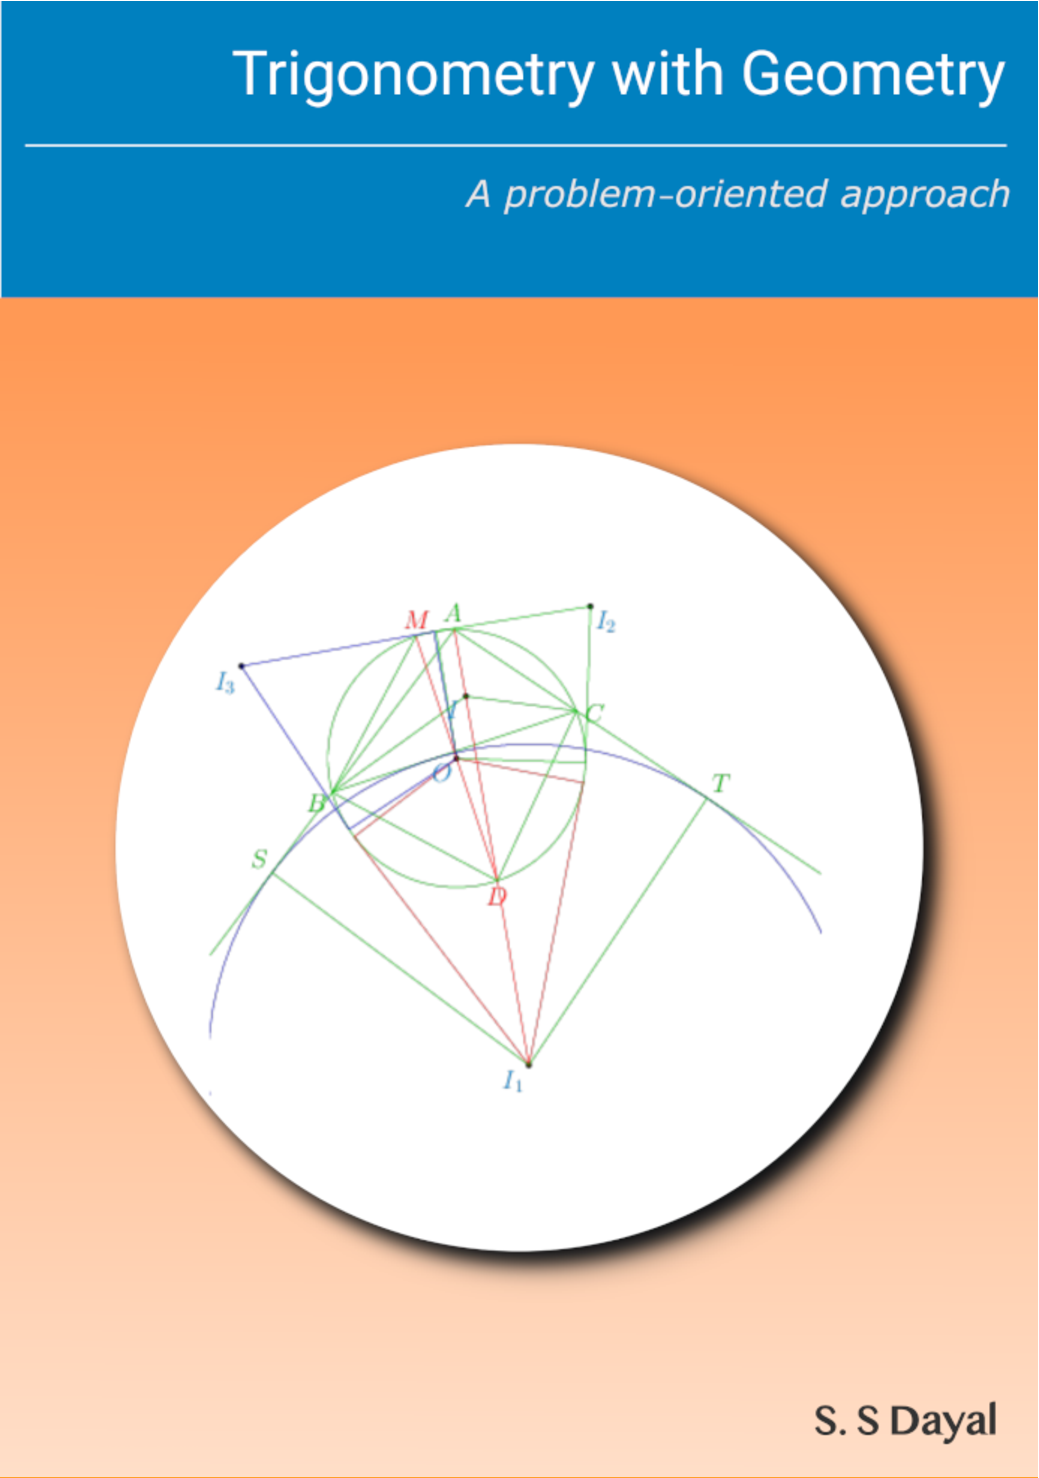
\includegraphics{cover.pdf}}
\titleformat{\section}
  {\normalfont\sffamily\Large\bfseries\color{nicecyan}}
  {\thesection}{0.2em}{}
\titleformat{\subsection}
  {\normalfont\sffamily\large\bfseries\color{nicecyan}}
  {\thesection}{0.2em}{}
\titleformat{\subsubsection}
  {\normalfont\sffamily\large\bfseries\color{nicecyan}}
  {\thesection}{0.2em}{}
\titleformat{\subsubsubsection}
  {\normalfont\sffamily\bfseries\color{nicecyan}}
  {\thesection}{0.2em}{}
\renewcommand{\ttdefault}{pcr}
\setlength{\parskip}{1em}
%\renewcommand{\rmdefault}{ptm}
%\renewcommand{\rmdefault}{phv}
\usepackage{fontspec}
%\setmainfont{TeX Gyre Pagella}
%\setmonofont[Ligatures=TeX,Scale=.90]{Courier}
\setsansfont{Roboto}
%\usepackage{unicode-math}
%\setmathrm{texgyrepagella-math.otf}
\newtheorem{remark}{Remark}[section]
\newtheorem{definition}{Definition}[section]
\newtheorem{proposition}{Proposition}[section]
\usepackage{polyglossia}

\setmainlanguage{english}
\setotherlanguages{sanskrit} %% or other languages

\newfontfamily\devanagarifont[Script=Devanagari]{Lohit Devanagari}
\renewcommand{\contentsname}{Table of Contents}
\makeindex
\setcounter{secnumdepth}{5}
\usepackage{etoolbox}
\makeatletter
\preto{\@verbatim}{\topsep=0pt \partopsep=0pt }
\makeatother
\begin{document}
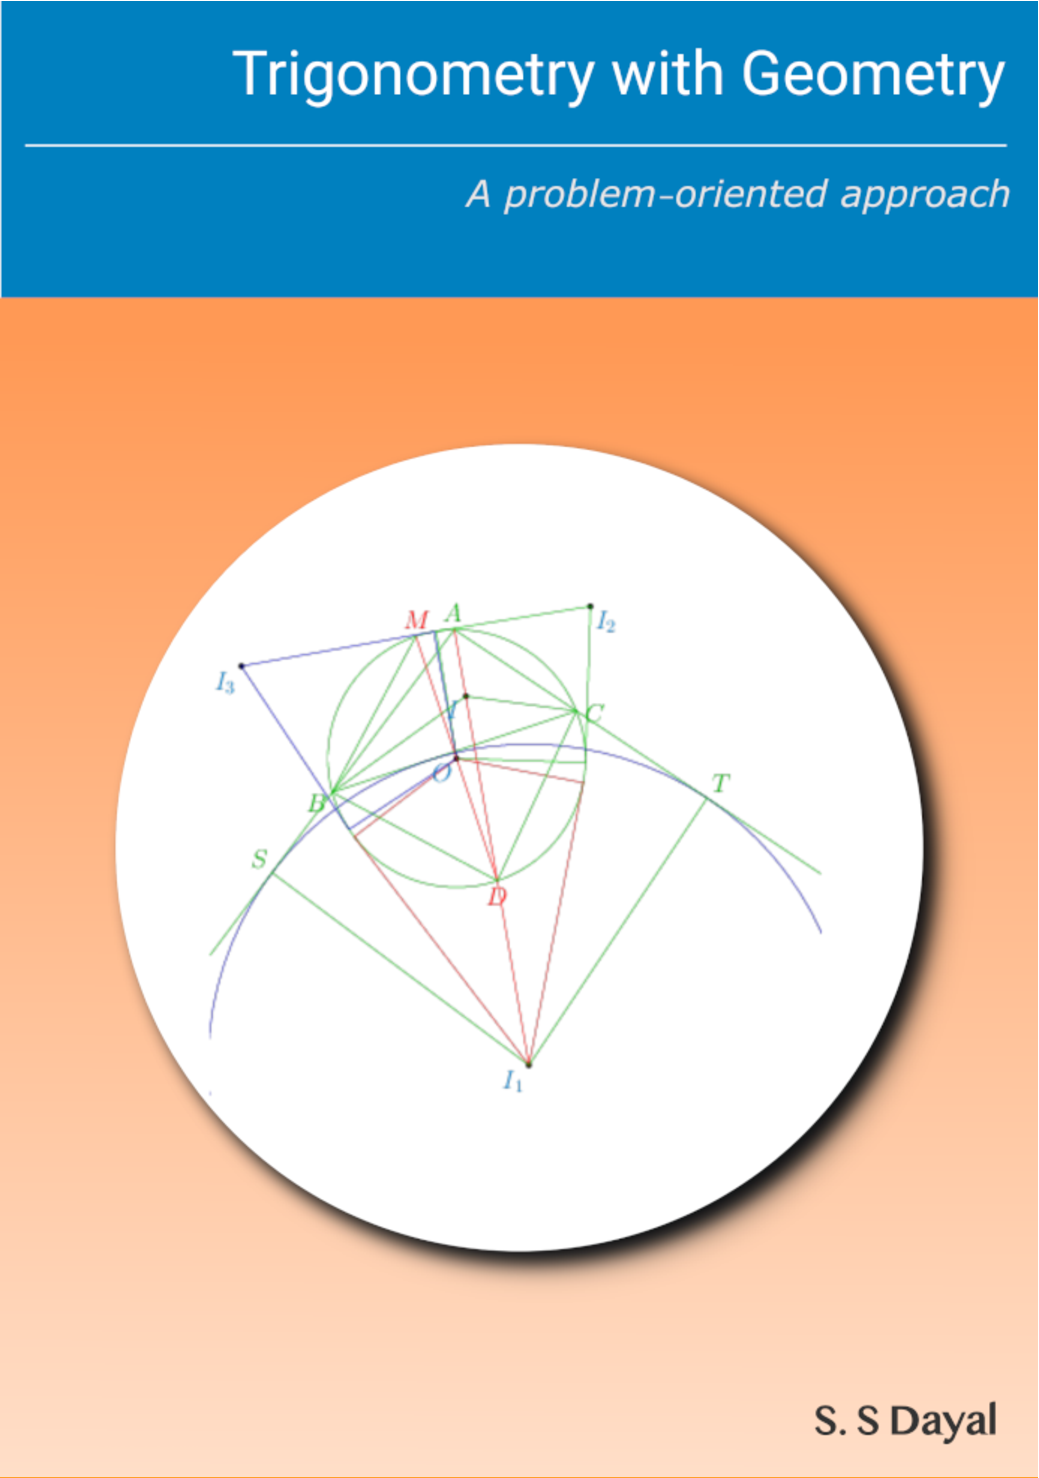
\includepdf[pages=1,fitpaper]{cover}
\thispagestyle{empty}
\pagestyle{empty}
\vfill
\newpage
\vspace*{5in}
Build Date: \today
\vspace*{0.2in}

Copyright, \copyright~ Shiv Shankar Dayal, 2011-2023. All rights reserved.\\\\
Permission is granted to copy, distribute and/or modify this document under the
terms of the GNU Free Documentation License, Version 1.3 or any later version
published by the Free Software Foundation; with no Invariant Sections, no
Front-Cover Texts, and no Back-Cover Texts. A copy of the license is included
in the section entitled ``GNU Free Documentation License''.
\newpage
\vspace*{2in}
\begin{center}
  \Large \it Dedicated to my family\\and Free Software Community
\end{center}
\vspace*{1cm}
\begin{center}
  \large When you take an action think of the poorest person you have seen and evaluate how
  your action will benefit that person.
\end{center}
\begin{center}
\begin{sanskrit}
  स्वध्याय परमो तपः
\end{sanskrit}
(Self study is ultimate penance.)
\end{center}
\newpage
% \newpage
% \listofpyglistings
\newpage
\frontmatter
\setcounter{page}{1}
\pagenumbering{roman}
\tableofcontents
\chapter{Preface}
This is a book on trigonometry, which, covers basics of trigonometry till high school level. It covers the most essential topics to
take up a bachelor's course where knowledge of trigonometry is required. There is no specific purpose for writing this book. This
is a book for self study and is not recommended for courses in schools and universities. I will try to cover as much as I can and
will keep adding new material over a long period. I have no interest in writing a book in a fixed way which serves a university or
college course as I have always loved freedom. Life, freedom and honor in that order are important. That was one of the reasons why
I never did a masters course. Enough of personal rant. Let us get on with the actual work.

Trigonomtery is probably one of the most fundamental subjects in Mathematics as further study of subjects like coordinate geometry,
3D and 2D geometry, engineerring and rest all depend on it. It is very important to understand trigonometry for the readers if they
want to advance further in mathematics.

\section*{Why I Wrote This Book?}
I wrote this book for myself! I did not write it for anybody else. My knowledge, which I have acquired by reading books written by
many great mathematicians and authors and interactions with many intelligent people, is what has been put in the book. I have just
tried to add my flavor to it. Think of it as notes for me. Just that I like to organize my notes so it has taken form of a book and
nothing more. If you benefit from this then that is a pure coincidence and not intentional at all.

\section*{How to Read This Book?}
No I will not simply tell that you must solve the problems. My advice would be more detailed. Every chapter will have theory. Read
that first. Make sure you understand that. Of course, you have to meet the prerequisites for the book. Then, go on and try to solve
the problems. In this book, there are no pure problems. Almost all have answers except those which are of similar kind and
repetitive in nature for the sake of practice. If you can solve the problem then all good else look at the answer and try to
understand that. Then, few days later take on the problem again. If you fail to understand the answer you can always email me with
your work and I will try to answer to the best of my ability. However, if you have a local expert seek his/her advice first. Just
that email is bad for mathematics.

Note that mathematics is not only about solving problems. If you understand the theory well, then you will be able to solve
problems easily. However, problems do help enforce with the enforcement of theory in your mind.

I am a big fan of old MIR publisher's problem books, so I emphasize less on theory and more on problems. I hope that you find
this style much more fun as a lot of theory is boring. Mathematics is about problem solving as that is the only way to
enforce theory and find innovtive techniques for problem solving.

Some of the problems in certain chapters rely on other chapters which you should look ahead or you can skip those problems and come
back to it later. Since this books is meant for self study answers of most of the problems have been given which you can make use of.
However, do not use for just copying but rather to develop understanding.

\section*{Who Should Read This Book?}
Since this book is written for self study anyone with interest in trigonometry can read it. That does not mean that school or
college students cannot read it. You need to be selective as to what you need for your particular requirements. This is mostly high
school course with a little bit of lower classes' course thrown in with a bit of detail here and there.

\section*{Prerequisite}
You should have knowledge till grade 10th course. Attempt has been made to keep it simple and give as much as background to the
topic which is reasonable and required. However, not everything will be covered below grade 10.

\section*{Goals for Readers}
The goal of for reading this book is becoming proficient in solving simple and basic problems of trigonometry. Another goal would
be to be able to study other subjects which require this knowledge like trigonometry or calculus or physics or chemistry or other
subjects. If you can solve 95\% problems after 2 years of reading this book then you have achieved this goal.

All of us possess a certain level of intelligence. At average any person can read this book. But what is most important is you have
to have interest in the subject. Your interest gets multiplied with your intelligence and thus you will be more capable than you
think you can be. One more point is focus and effort. It is not something new which I am telling but I am saying it again just to
emphasize the point. Trust me if you are reading this book for just scoring a nice grade in your course then I have failed in my
purpose of explaining my ideas.

Also, if you find this book useful feel free to share it with others without hesitation as it is free as in freedom. There are no
conditions to share it.

\section*{Acknowledgements}
I am in great debt of my family and free software community because both of
these groups have been integral part of my life. Family has prvided direct
support while free software community has provided the freedom and freed me
from the slavery which comes as a package with commercial software. I am
especially grateful to my wife, son and parents because it is their time which
I have borrowed to put in the book. To pay my thanks from free software
community  I will take one name and that is Richard Stallman who started all
this  and is still fighting this never-ending war. When I was doing the algebra
book then I realized how difficult it is to put Math on web in HTML format and
why Donald Knuth wrote \TeX{}. Also, \TeX{} was one of the first softwares to
be released as a free software.

Now as this book is being written using \LaTeX{} so obviously Leslie Lamport
and all the people involved with it have my thanks along with Donald Knuth. I
use Emacs with Auctex and hope that someday I will use it in a much more
productive way someday.

I have used Asymptote and tikz for drawing all the diagrams. Both are wonderful
packages and work very nicely. Asymptote in particular is very nice for 3d-drawings and linear equation solving.

I would like to thank my parents, wife and son for taking out their fair share
of time and the support which they have extended to me during my bad
times. After that I would like to pay my most sincere gratitude to my teachers
particularly H. N. Singh, Yogendra Yadav, Satyanand Satyarthi, Kumar Shailesh
and Prof. T. K. Basu. Now is the turn of people from software community. I must
thank the entire free software community for all the resources they have
developed to make computing better. However, few names I know and here they
go. Richard Stallman is the first, Donald Knuth, Edger Dijkstra, John von Neumann after that as their lives have strong influence in
how I think and base my life on. Cover graphics has been done by Koustav Halder so much thanks to him.

I am not a native English speaker and this book has just gone through one pair
of eyes therefore chances are high that it will have lots of errors(particularly with commas and spelling mistakes). At the
same time it may contain lots of technical errors. Please feel free to drop me
an email at
\href{mailto:shivshankar.dayal@gmail.com}{shivshankar.dayal@gmail.com} where I
will try to respond to each mail as
much as possible. Please use your real names in email not something like
coolguy. If you have more problems which you want to add it to the book please send
those by email or create a PR on github. The github url is \url{https://github.com/shivshankardayal/Trigonometry-Latex}.
\begin{flushright}
Shiv Shankar Dayal
\end{flushright}

\newpage
\pagestyle{fancy}
\mainmatter
\pagenumbering{arabic}
\part{Theory and Problems}
\chapter{Measurement of Angles}
The word trigonometry comes from means measurement of triangles. The word originally comes from Greek language.
measurement. The objective of studying plane trigonometry is to develop a method of solving plane triangles. However, as time
changes everything it has changed the scope of trigonometry to include polygons and circles as well. A lot of concepts in this book
will come from your geometry classes in lower classes. It is a good idea to review the concepts which you have studied till now
without which you are going to struggle while studying trigonometry in this book.

\section{Angles in Geometry}
If we consider a line extending to infinity in both directions, and a point $OO$ which divides this line in two parts one on each
side of the point then each part is called a ray or half-line. Thus $O$ divides the line into two rays $OA$ and $OA'$.

\begin{center}
  \begin{tikzpicture}
    \draw[>=latex,<->] (0, 0) -- (3, 0);
    \draw (.5, -.1) -- (.5, .1);
    \draw (.5,0) node[anchor=north] {$A'$};
    \draw (2.5, -.1) -- (2.5, .1);
    \draw (2.5,0) node[anchor=north] {$A$};
    \draw (1.5, -.1) -- (1.5, .1);
    \draw (1.5,0) node[anchor=north] {$O$};
  \end{tikzpicture}
\end{center}

The point $O$ is called vertex or origin for these days. An angle is a figure formed by two rays or half lies meeting at a common
vertex. These half lines are called {\it sides of the angle}.

An angle is denoted by the symbol $\angle$ followed by three capital letters of which the middle one represents the vertex and
remaining two points point to two sides. Otherwise the angle is simply written as one letter representing the vertex of the
angle.

\begin{center}
  \begin{tikzpicture}
    \draw[->, >=stealth] (0,0) -- (2,0);
    \draw[->, >=stealth] (0,0) -- (1, 1.732);
    \draw (0.3, 0) arc [start angle=0, end angle=60, radius=0.3];
    \draw (2, 0) node[anchor=north] {$A$};
    \draw (1, 1.732) node[anchor=north west] {$B$};
    \draw (0, 0) node[anchor=north] {$O$};
  \end{tikzpicture}
\end{center}


The angle in above image is written as $\angle AOB$ or $\angle BOA$ or $\angle O$.

Each angle can be measured and there are different units for the measurement. In Geometry, an angle always lie between $0^\circ$
and $360^\circ$ and negative angles are meaningless. Measure of an angle is the smallest amount of rotation from the direction of
one ray of the angle to the direction of the other.

\section{Angles in Trigonometry}
Angles are more generalized in Trigonometry. They can have positive or negative values. As was the case in gerometry, similarly
angles are measured in Trigonometry. The starting and ending positions of revolving rays are called initial side and terminal side
respectively. The revolving half line is called the generating line or the radius vector. For example, if $OA$ and $OB$ are the
initial and final position of the radius vector then angle formed will be $\angle AOB$.

\section{Angles Exceeding $360^\circ$}
\begin{center}
  \begin{tikzpicture}
	  \draw [->]( 0,0) -- (4,0);
	  \draw [->]( 0,0) -- (0,4);
	  \draw [->,red]( 0,0) -- (400:4);
    \draw[->,domain=0:400,variable=\t,samples=200,>=latex]
    plot ({(\t+400)*cos(\t)/(400)},
    {(\t+400)*sin(\t)/(400)}) node[right=.5cm] {$400^\circ$};
  \end{tikzpicture}
\end{center}

In Geometry, angles are limited to $0^\circ$ to $360^\circ$. However, when multiple revolutions are involved angles are more than
$360^\circ$. For example, the revolving line starts from the initial position and makes $n$ complete revolutions in anticlockwise
direction and also further angle $\alpha$ in the same direction. We then have a certain angle $\beta_n$ given by $\beta_n =
x\times360^\circ + \alpha$, where $0^\circ< \alpha < 360^\circ$ and $n$ is zero or positive integer. Thus, there are infinite
possible angles.

Angles formed by anticlockwise rotation of the radius vector are taken as positive and angles formed by clockwise rotation of the
radius vector are taken as negative.

\section{Quadrants}
\begin{center}
  \begin{tikzpicture}
    \draw[>=latex,<->] (0, 0) -- (3, 0);
    \draw (0,0) node[anchor=north] {$X'$};
    \draw (3,0) node[anchor=north] {$X$};
    \draw (1.5,0) node[anchor=north east] {$O$};
    \draw[>=latex,<->] (1.5, -1.5) -- (1.5, 1.5);
    \draw (1.5, -1.5) node[anchor=west] {$Y'$};
    \draw (1.5, 1.5) node[anchor=west] {$Y$};
  \end{tikzpicture}
\end{center}

Let $XOX'$ and $YOY'$ be two mutually perpendicular lines in a plane and $OX$ be the initial half line. The lines divide the whole
reason in quadrants. $XOY, YOX', X′OY$' and $Y′OX$ are respectively called $1$st, $2$nd, $3$rd and $4$th quadrants. According to
terminal side lying in $1$st, $2$nd, $3$rd and $4$th quadrants the angles are said to be in $1$st, $2$nd, $3$rd and $4$th quadrants
respectively. A {\it quandrant angle} is an angle formed if terminal side coincides with one of the axes.

For any angle $\angle$ which is not a quadrant angle and when number of revolutions is zero and radius vector rotates in
anticlockwise directions:

\begin{enumerate}
\item $0^\circ< \alpha < 90^\circ$ if $\alpha$ lies in first quadrant
\item $90^\circ< \alpha < 180^\circ$ if $\alpha$ lies in second quadrant
\item $180^\circ< \alpha < 270^\circ$ if $\alpha$ lies in third quadrant
\item $270^\circ< \alpha < 360^\circ$ if $\alpha$ lies in fourth quadrant
\item when terminal side lies on $OY$, angle formed $=90^\circ$
\item when terminal side lies on $OX'$, angle formed $=180^\circ$
\item when terminal side lies on $OY'$, angle formed $=270^\circ$
\item when terminal side lies on $OX$, angle formed $=360^\circ$
\end{enumerate}

\section{Units of Measurement}
In Geometry, angles are usually measured in terms of right angles, however, that is an inconvenient system for smaller angles. So
we introduce different systems of measurements. There are three system of units for this:

\begin{enumerate}
\item Sexagecimal or British system: In British system, a right angle is divided into $90$ equal parts called degrees. Each degree
is then divided into $60$ equal parts called minutes and each minute is further is divided into $60$ parts called seconds.

A degree, a minute and a second are denoted by $1^\circ, 1"$, and $1$ respectively.
\item Centesimal or French System: In French system, a right angle is divided into $100$ equal parts called grades. Each grade is
then divided into $100$ equal parts called minutes and each minute is further is divided into $100$ parts called seconds.

A degree, a grade and a second are denoted by $1^g, 1"$, and $1$ respectively.
\item Radian or Circular Measure: An arc equal to radius of a circle when subtends an anngle on the center then that angle is $1$
radian and is denoted by $1^c$. The angle made by half of perimeter is $\pi$ radians. Also, from Geometry we know that angle subtended
is the ratio between length of cord and radius. This ratio is in radians. Since both length or chord and radius have same unit
radian is a constant.
\end{enumerate}

\subsection{Relationship between Systems of Measurements}
If measure of an angle if $D$ degrees, $G$ grades and $C$ radians then upon elementary manipulation we find that $\frac{D}{180}=
\frac{G}{200} = \frac{C}{\pi}$.

\subsection{Meaning of $\pi$}
The ratio of circumference and diameter of a circle is always constant and this constant is denoted by gree letter $\pi$.

$\pi$ is an irrational number. In general, we use the value of $\frac{22}{7}$ but $\frac{355}{113}$ is more accurate though not
exact. If $r$ be the radius of a circle and $c$ be the circumference then $\frac{c}{2r} =\pi$ leading circumference to be $c = 2\pi
r$.

\section{Problems}
\begin{enumerate}
\item Reduce $63^{\circ}14'51''$ to centisimal measure.
\item  Reduce $`45^{\circ}20'10''$ to centisimal and radian measure.
\item Reduce $94^g23'27''$ to Sexagecimal measure.
\item Reduce $1.2$ radians in Sexageciaml measure.
\end{enumerate}

Express in terms of right angle; the angles

\begin{enumerate}[resume]
\item $60^{\circ}$
\item $75^{\circ}15'$
\item $63^{\circ}17'25''$
\item $130^{\circ}30'$
\item $210^{\circ}30'30''$
\item $370^{\circ}20'48''$
\end{enumerate}

Express in grades, minutes and degrees

\begin{enumerate}[resume]
\item $30^{\circ}$
\item $81^{\circ}$
\item $138^{\circ}30'$
\item $35^{\circ}47'15''$
\item $235^{\circ}12'36''s$
\item $475^{\circ}13'48''$
\end{enumerate}

Express in terms of right angles and also in degrees, minutes and seconds; the angles

\begin{enumerate}[resume]
\item $120^g$
\item $45^g35'24''$
\item $39^g45'36''$
\item $255^g8'9''$
\item $759^g0'5''$
\item Reduce $55^{\circ}12'36''$ to centisimal measure.
\item Reduce $18^{\circ}33'45''$ to circular measure.
\item Reduce $196^g35'24''$ to sexagecimal measure.
\item How many degrees, minutes and seconds are respectively passed over in $11\frac{1}{9}$ minutes by the hour and minute hand
    of a watch.
\item The number of degrees in one acute angle of a right-angled triangle is equal to the number of grades in the other; express both
    angles in degrees.
\item Prove that the number of Sexagecimal minutes in any angle is to the number of Centisimal minutes in the same angle as
    $27:50.$
\item Divide $44^{\circ}8'$ into two parts such that the number of Sexagecimal seconds in one part may be equal to number of
    Centisimal seconds in the other part.
\item The angles of a triangle are in the ratio of $3:4:5$, find the smallest angle in degrees and greatest angle in radians.
\item Find the angle between the hour hand and the minute hand in circular measure at half past four.
\item If $p, q$ and $r$ denote the grade measure, degree measure and the radian measure of the same angle, prove that
  \begin{enumerate}
    \item $\frac{p}{10} = \frac{q}{9} = \frac{20r}{\pi}$
    \item $p - q = \frac{20r}{\pi}$
  \end{enumerate}
\item Two angles of a triangle are $72^{\circ}53'51''$ and $41^{\circ}22'50''$ respectively. Find the third angle in
    radians.
\item The angles of triangle are in A.P. and the number of radians in the greatest angle is to the number of degrees in the least one
    as $\pi:60$; find the angles in degrees.
\item The angles of a triangle are in A.P. and the number of grades in the least is to the number of radians in the greatest is
$40:\pi$; find the angles in degrees.
\item Three angles are in G.P. The number of grades in the greatest angle is to the number of circular units in the least is
    $800:\pi$; and the sum of angles is $126^\circ$. Find the angles in grades.
\item Find the angle between the hour-hand and minute-hand in circular measure at $4$ o'clock.
\item Express in sexagecimal system the angle between the minute-hand and hour-hand of a clock at quarter to twelve.
\item The diamter of a wheel is $28$ cm; through what distance does its center move during one rotation of wheel along the
    ground?
\item What must be the radius of a circular running path, round which an athlete must run $5$ time in order to describe
    $1760$ meters?
\item The wheel of a railway carriage is $90$ cm in diameter and it makes $3$ revolutions per second; how fast is the
    train going?
\item A mill sail whose length is $540$ cm makes $10$ revolutions per minute. What distance does its end travel in one
    hour?
\item Assuming that the earth describes in one year a circle, or $149,700,000$ km. radius, whose center is the sun, how many
    miles does earth travel in a year?
\item The radius of a carriage wheel is $50$ cm, and in $\frac{1}{9}$ th of a second it turns through $80^\circ$
    about its center, which is fixed; how many km. does a point on the rim of the wheel travel in one hour?
\item Express in terms of three systems of angular measurements the magnitude of an angle of a regular decagon.
\item One angle of a triangle is $\frac{2}{3}x$ grades and another is $\frac{3}{2}x$ degrees, while the third is
    $\frac{\pi x}{75}$ radians; express them all in degrees.
\item The circular measure of two angles of a triangle are $\frac{1}{2}$ and $\frac{1}{3}$. What is the number of degrees
    of the third angle?
\item The angles of a triangle are in A.P. The number of radians in the least angle is to the number of degree in the mean angle is
    $1:120$. Find the angles in radians.
\item Find the magnitude, in radians and degrees, of the interior angle of 1. a regular pentagon 2. a regular heptagon 3. a regualr
    octagon 4. a regular duodecagon 5. a polygon with $17$ sides
\item The angle in one regular polygon is to that in another is $3:2$, also the number of sides in the first is twice that in
    the second. How many sides are there in the polygons?
\item The number of sides in two regular polygons are as $5:4$, and the difference between their angles is $9^\circ$;
    find the number of sides in the polygons.
\item Find two regular polygons such that the number of their sides may be $3$ to $4$ and the number of degrees of an
    angle of the first to the number of grades of the second as $4$ to $5.$
\item The angles of a qadrilateral are in A.P. and the greatest is double the least; express the least angle in radians.
\item Find in radians, degrees, and grades the angle between hour-hand and minute-hand of a clock at 1. half-past three 2. twenty
    minutes to six 3. a quarter past eleven.
\item Find the times 1. between fours and five o'clock when the angle between the minute hand and the hour-hand is
    $78^\circ,$ 2. between seven and eight o'clock when the angle is $54^\circ$
\item The interior angles of a polygon are in A.P. The smallest angle is $120^\circ$ and the common difference is
    $5^\circ$. Find the number of sides of the polygon.
\item The angles of quadrilateral are in A.P. and the number of grades in the least angle is to the number of radians in the greatest is
    $100:\pi$. Find the angles in degrees.
\item The anlges of a polygons are in A.P. The least angle is $\frac{5\pi}{12}$ common difference is $10^\circ$, find the
    number of sides in the polygon.
\item Find the angle subtended at the center of a circle of radius $3$ cm. by an arc of length $1$ cm.
\item In a circle of radius $5$ cm., what is the length of the arc which subtends an angle of $33^\circ15'$ at the center.
\item Assuming the average distance of sun from the earth to be $149,700,000$ km., and the angle subtended by the sun at the
    eye of a person on the earth is $32'$, find the sun's diameter.
\item Assuming that a person of normal sight can read print at such a distance that the letter subtends and angle of $5'$ at
    his eye, find what is the height of the letters he can read at a distance of 1. $12$ meters 2. $1320$ meters.
\item Find the number of degrees subtended at the center of a circle by an arc whose length is $0.357$ times the radius.
\item Express in radians and degrees the angle subtended at the center of a circle by an arc whose length is $15$ cm., the
    radius of the circle being $25$ cm.
\item The value of the divisions on the outer rim of a graduated cicle is $5'$ and the distance between successive graduations
    is $.1$ cm. Find the radius of the circle.
\item The diamter of a graduated circle is $72$ cm., and the gradiuations on the rim are $5'$ apart; find the distance of
    one graduation to to another.
\item Find the radius of a globe which is such that the distance between two places on the same meridian whose latitude differs by
    $1^\circ10'$ may be $0.5$ cm.
\item Taking the radius of earth to as $6400$ km., find the difference in latitude of two places, one of which is $100$
    km. north of another.
\item Assuming the earth to be a sphere and the difference between two parallels of latitude, which subtends an angle of
    $1^\circ$ at the eath's center, to be $69\frac{1}{2}$ km., find the radius of the earth.
\item What is the ratio of radii of the circles at the center of which two arcs of same length subtend angles of $60^\circ$ and
    $75^\circ$?
\item If an arc, of length $10$ cm., on a circle of $8$ cm. diameter subtend at the center of circle an angle of
    $143^\circ14'22''$, find the value of $\pi$ to $4$ places of decimals.
\item If the circumference of a circle be divided into five parts which are in A.P., and if the greatest part be six times the least
    find in radians the the magnitude of the angles the parts subtend at the center of the circle.
\item The perimeter of a certain sector of a circle is equal to the length of the arc of a semicircle having the same radius; express
    the angle of the sector in degrees.
\item At what distance a man, whose height is $2$ m., subtend an angle of $10'$.
\item Find the length which at a distance of $5280$ m., will subtend an angle of $1'$ at the eye.
\item Assuming the distance of the earth from the moon to be $38400$ km., and the angle subtended by the moon at the eye of a
    person on earth to be $31'$, find the diameter of the moon.
\item The wheel of a railway carriage is $4$ ft. in diameter and makes $6$ revolutions in a second; how fast is the train
    going?
\item Assuming that moon subtends an angle of $30'$ at the eye of an observer, find how far from the eye a coin of one inch
    diameter must be held so as just to hide the moon.
\item A wheel make $30$ revolutions per minute. Find the circular measure of the angle described by spoke in half a second.
\item A man running along a circular track at the rate of $10$ miles per hour, traverses in $36$ seconds, an arc which
    subtends an angle of $56^\circ$ at the center. Find the diamter of the circle.
\end{enumerate}

\chapter{Trigonometric Ratios}
From Geometry, we know that an acute angle is an angle whose measure is between $0^\circ$ and $90^\circ$. Consider the following
figure:
\begin{center}
  \begin{tikzpicture}
    \draw (0, 0) -- (4, 0);
    \draw (0, 0) -- (4, 4);
    \draw (2, 2) -- (2, 0);
    \draw (3, 3) -- (3, 0);
    \draw [blue] (0,0) node[anchor=north east] {$O$};
    \draw [blue] (2,0) node[anchor=north] {$M$};
    \draw [blue] (3,0) node[anchor=north] {$M'$};
    \draw [blue] (2,2) node[anchor=south east] {$P$};
    \draw [blue] (3,3) node[anchor=south east] {$P'$};
  \end{tikzpicture}
\end{center}

This picture contains two similar triangles $\triangle OMP$ and $\triangle OM'P'$. We are interested in $\angle MOP$ or $\angle
M'OP'0$. In the $\triangle MOP$ and $\triangle M'OP', OP, OP'$ are called the hypotenuses i.e. sides opposite to the right angle,
$PM, P'M'$ are called perpendiculars i.e. sides opposite to the angle of interest and $OM, OM'$ are called bases i.e. the third
angle.

Hypotenuses are usually denoted by $h$, perpendiculars by $p$ and bases by $b$. Let $OM = b, OM' = b', PM=p, P'M' = p', OP = h, OP'
= h'$. Since the two triangles are similar $\therefore \frac{p}{p'} = \frac{b}{b'} = \frac{h}{h'}$. Thus rhe ratio of any two sides
is dependent purely on $\angle O$ or $\angle MOP$ or $\angle M'OP'$.

Since there are three sides, we can choose $2$ in ${}^3C_2$ i.e. $3$ ways and for each combination there will be two permutations
where a side can be in either numerator or denominator. From this we can conclude that there will be six ratios(these are called
trigonometric ratios), These six trigonometric ratios or functions are given below:

$\dfrac{MP}{OP}$ or $\dfrac{p}{h}$ is called the {\bf Sine} of the $\angle MOP$.

$\dfrac{OM}{OP}$ or $\dfrac{b}{h}$ is called the {\bf Cosine} of the $\angle MOP$.

$\dfrac{MP}{OM}$ or $\dfrac{p}{b}$ is called the {\bf Tangent} of the $\angle MOP$.

$\dfrac{OP}{MP}$ or $\dfrac{h}{p}$ is called the {\bf Cosecant} of the $\angle MOP$.

$\dfrac{OP}{OM}$ or $\dfrac{h}{b}$ is called the {\bf Secant} of the $\angle MOP$.

$\dfrac{OM}{MP}$ or $\dfrac{b}{p}$ is called the {\bf Cotangent} of the $\angle MOP$.

$1 - \cos MOP$ is called the {\bf Versed Sine} of $\angle MOP$ and $1 - \sin MOP$ is called the {\bf Coversed Sine} of $\angle
MOP$. These two are rarely used in trigonometry. It should be noted that the trigonometric ratios are all numbers. The name of the
trigonometric ratios are written for brevity $\sin MOP, \cos MOP, \tan MOP, \cot MOP, \sec MOP, {\rm cosec}~MOP, {\rm vers}~MP,
{\rm coverse}~MOP$.

\section{Relationship betweeen Trigonometric Functions or Ratios}
Let us represent the $\angle MOP$ with $\theta$, we observe from previous section that
$$\sin\theta = \dfrac{1}{\csc\theta}, \cos\theta = \frac{1}{\sec\theta}, \tan\theta =
\frac{1}{\cos\theta}, {\rm cosec}\theta = \frac{1}{\sin\theta}, \sec\theta = \frac{1}{\cos\theta}, \cot\theta =
\frac{1}{\tan\theta}$$

We also observe that $\tan\theta = \dfrac{\sin\theta}{\cos\theta}$ and $\cot\theta = \dfrac{\cos\theta}{\sin\theta}$

From Pythagora theorem in geometry, we know that ${\rm hypotenuse}^2 = {\rm perpendicular}^2 + {\rm base}^2$ or $h^2 = p^2 + b^2$

\begin{enumerate}
\item Dividing both side by $h^2$, we get

$$ \dfrac{p^2}{h^2} + \dfrac{b^2}{h^2} = 1$$
$$ \sin^2\theta + \cos^2\theta = 1$$

We can rewrite this as $\sin^2\theta = 1 - \cos^2\theta, \cos^2\theta = 1 - \sin^2\theta, \sin\theta = \sqrt{1 - \cos^2\theta},
\cos\theta = \sqrt{1 - \sin^2\theta}$.

\item If we divide both sides by $b^2$, then we get

$$ \frac{h^2}{b^2} = \frac{p^2}{b^2} + 1 $$
$$ \sec^2\theta = \tan^2\theta + 1$$

We can rewrite this as $\sec^2\theta - \tan^2\theta = 1, \tan^\theta = \sec^2\theta - 1, \sec\theta = \sqrt{1 + \tan^2\theta},
\tan\theta = \sqrt{sec^2\theta - 1}$

\item Similalry, if we divide by $p^2$, then we get

$$ \frac{h^2}{p^2} = 1 + \frac{b^2}{p^2}$$
$$ {\rm cosec}^2\theta = 1 + \cos^2\theta$$

We can rewrite this as ${\rm cosec}^2\theta - \cot^2\theta = 1, \cot^2\theta = {\rm cosec}^2\theta - 1, {\rm cosec}\theta = \sqrt{1 +
\cot^2\theta}, \cot\theta = \sqrt{{\rm cosec}^2\theta - 1}$
\end{enumerate}

\section{Problems}
Prove the following:

\begin{enumerate}
\item $\sqrt{\frac{1 - \cos A}{1 + \cos A}} = {\rm cosec} A - \cot A$.
\item $\sqrt{\sec^2A + {\rm cosec}^2A} = \tan A + \cot A$.
\item $({\rm cosec} A - \sin A)(\sec A - \cos A)(\tan A + \cot A) = 1$.
\item $\cos^4 A - \sin^4 A + 1 = 2\cos^2 A$.
\item $(\sin A + \cos A)(1 - \sin A\cos A) = \sin^3A + \cos^3A$.
\item $\frac{\sin A}{1 + \cos A}+\frac{1 + \cos A}{\sin A} = 2{\rm cosec} A$.
\item $\sin^6A - cos^6A = 1 - 3\cos^2A\sin^2A$.
\item $\sqrt{\frac{1 - \sin A}{1 + \sin A}} = \sec A - \tan A$.
\item $\frac{{\rm cosec} A}{{\rm cosec} A - 1} + \frac{{\rm cosec} A}{{\rm cosec} A + 1} = 2\sec^2 A$.
\item $\frac{{\rm cosec} A}{\tan A + \cot A} = \cos A$.
\item $(\sec A + \cos A)(\sec A - \cos A) = \tan^2 A + \sin^2A$.
\item $\frac{1}{\tan A + \cot A} = \sin A\cos A$.
\item $\frac{1 - \tan A}{1 + \tan A} = \frac{\cot A - 1}{\cot A + 1}$.
\item $\frac{1 + \tan^2A}{1 + \cot^2A} = \frac{\sin^2A}{\cos^2A}$.
\item $\frac{\sec A - \tan A}{\sec A + \tan A} = 1 - 2\sec A\tan A + 2\tan^2 A$.
\item $\frac{1}{\sec A - \tan A} = \sec A + \tan A$.
\item $\frac{\tan A}{1 - \cot A} + \frac{\cot A}{1 - \tan A} = \sec A{\rm cosec} A+ 1$.
\item $\frac{\cos A}{1 - \tan A} + \frac{\sin A}{1 - \cot A} = \sin A + \cos A$.
\item $(\sin A + \cos A)(\tan A + \cot A) = \sec A + {\rm cosec} A$.
\item $\sec^4A - \sec^2A = \tan^4A + \tan^2A$.
\item $\cot^4A + \cot^2A = {\rm cosec}^4A - {\rm cosec}^2A$.
\item $\sqrt{{\rm cosec}^2A - 1} = \cos A{\rm cosec} A$.
\item $\sec^2A{\rm cosec}^2A = \tan^2A + \cot^2A + 2$.
\item $\tan^2A - \sin^2A = \sin^4A \sec^2A$.
\item $(1 + \cot A - {\rm cosec} A)(1 + \tan A + \sec A) = 2$.
\item $\frac{\cot A\cos A}{\cot A + \cos A} = \frac{\cot A - \cos A}{\cot A \cos A}$.
\item $\frac{\cot A + \tan B}{\cot B + \tan A} = \cot A \tan B$.
\item $\left(\frac{1}{\sec^2 A - \cos^2A} + \frac{1}{{\rm cosec}^2A - \sin^2A}\right)\cos^2A\sin^2A = \frac{1 - \cos^2A\sin^2A}{2 +
    \cos^2A\sin^2A}$.
\item $\sin^8A - \cos^8A = (\sin^2A - \cos^2A)(1 - 2\sin^2A\cos^2A)$.
\item $\frac{\cos A{\rm cosec} A - \sin A\sec A}{\cos A + \sin A} = {\rm cosec} A - \sec A$.
\item $\frac{1}{{\rm cosec} A - \cot A} - \frac{1}{\sin A} = \frac{1}{\sin A} - \frac{1}{{\rm cosec} A + \cot A}$.
\item $\frac{\tan A + \sec A - 1}{\tan A - \sec A + 1} = \frac{1 + \sin A}{\cos A}$.
\item $(\tan A + {\rm cosec} B)^2 - (\cot B - \sec A)^2 = 2\tan A\cot B({\rm cosec} A + \sec B)$.
\item $2\sec^2 A - \sec^4A - 2{\rm cosec}^2A + {\rm cosec}^4A = \cot^4A - \tan^4A$.
\item $(\sin A + {\rm cosec} A)^2 + (\cos A + \sec A)^2 = \tan^2A + \cot^2A + 7$.
\item $({\rm cosec} A + \cot A)(1 - \sin A) - (\sec A + \tan A)(1 - \cos A) = ({\rm cosec} A - \sec A)[2 - (1 - \cos A)(1 - \sin A)]$.
\item $(1 + \cot A + \tan A)(\sin A - \cos A) = \frac{\sec A}{{\rm cosec}^2A} - \frac{{\rm cosec} A}{\sec^2A}$.
\item $\frac{1}{\sec A - \tan A} - \frac{1}{\cos A} = \frac{1}{\cos A} - \frac{1}{\sec A + \tan A}$.
\item $3(\sin A - \cos A)^4 + 4(\sin^6 A + \cos^6 A) + 6(\sin A + \cos A)^2 = 13$.
\item $\sqrt{\frac{1 + \cos A}{1 - \cos A}} = {\rm cosec} A + \cot A$.
\item $\frac{\cos A}{1 + \sin A} + \frac{\cos A}{1 - \sin A} = 2\sec A$.
\item $\frac{\tan A}{\sec A - 1} + \frac{\tan A}{\sec A + 1} = 2{\rm cosec} A$.
\item $\frac{1}{1 - \sin A} - \frac{1}{1 + \sin A} = 2\sec A\tan A$.
\item $\frac{1 + \tan^2 A}{1 + \cot^2 A} = \left(\frac{1 - \tan A}{1 - \cot A}\right)^2$.
\item $1 + \frac{2\tan^2 A}{\cos^2 A} = \tan^4 A + sec^4 A$.
\item $(1 - \sin A - \cos A)^2 = 2(1 - \sin A)(1 - \cos A)$.
\item $\frac{\cot A + {\rm cosec} A - 1}{\cot A - {\rm cosec} A + 1} = \frac{1 + \cos A}{\sin A}$.
\item $(\sin A + \sec A)^2 + (\cos A + {\rm cosec} A)^2 = (1 + \sec A{\rm cosec} A)^2$.
\item $\frac{2\sin A\tan A(1 - \tan A) + 2\sin A\sec^2A}{(1 + \tan A)^2} = \frac{2\sin A}{1 + \tan A}$.
\item If $2\sin A = 2 - \cos A,$ find $\sin A$.
\item If $8\sin A = 4 + \cos A,$ find $\sin A$.
\item If $\tan A + \sec A = 1.5,$ find $\sin A$.
\item If $\cot A + {\rm cosec} A = 5,$ find $\cos A$.
\item If $3\sec^4 A + 8 = 10\sec^2A,$ find the value of $\tan A$.
\item If $\tan^2A + \sec A = 5,$ find $\cos A$.
\item If $\tan A + \cot A = 2,$ find $\sin A$.
\item If $\sec^2A = 2 + 2\tan A,$ find $\tan A$.
\item If $\tan A = \frac{2x(x + 1)}{2x + 1},$ find $\sin A$ and $\cos A$.
\item If $3\sin A + 5\cos A = 5,$ show that $5\sin A - 3\cos A = \pm 3$.
\item If $\sec A + \tan A = \sec A - \tan A$ prove that each side is $\pm 1$.
\item If $\frac{\cos^4 A}{\cos^2 B} + \frac{\sin^4 A}{\sin^2 B} = 1,$ prove that
  \begin{enumerate}
    \item $\sin^4A + \sin^4B = 2\sin^2A \sin^2B$,
    \item $\frac{\cos^4 B}{\cos^2 A} + \frac{\sin^4 B}{\sin^2 A} = 1$.
  \end{enumerate}
\item If $\cos A + \sin A = \sqrt{2}\cos A,$ prove that $\cos A - \sin A = \pm \sqrt{2}\sin A$.
\item If $a\cos A - b\sin A = c,$ prove that $a\sin A + b\cos A = \sqrt{a^2 + b ^2 - c^2}$.
\item If $1 - \sin A = 1 + \sin A,$ then prove that value of each side is $\pm \cos A$.
\item If $\sin^4 A + \sin^2 A = 1,$ prove that
  \begin{enumerate}
    \item $\frac{1}{\tan^4 A} + \frac{1}{\tan^2A} = 1$,
    \item $\tan^4A - \tan^2 = 1$.
  \end{enumerate}
\item If $\cos^2A - \sin^2 A = \tan^2 B,$ prove that $2\cos^2B - 1 = \cos^2B - \sin^2B = \tan^2A$.
\item If $\sin A + {\rm cosec} A = 2,$ then prove that $\sin^nA + {\rm cosec}^nA = 2$.
\item If $\tan^2A = 1 - e^2$, prove that $\sec A + \tan^3A {\rm cosec}A = (2 - e^2)^{\frac{3}{2}}$.
\item Eliminate $A$ between the equations $a\sec A + b\tan A + c = 0$ and $p\sec A + q\tan A + r = 0$.
\item If ${\rm cosec} A - \sin A = m$ and $\sec A - \cos A = n,$ elimiate $A$.
\item Is the equation $\sec^2 A = \frac{4xy}{(x + y)^2}$ possible for real values of $x$ and $y$?.
\item Show that the equation $\sin A = x + \frac{1}{x}$ is imossible for real values of $x$.
\item If $\sec A - \tan A = p, p\neq 0,$ find $\tan A, \sec A$ and $\sin A$.
\item If $\sec A = p + \frac{1}{4p},$ show that $\sec A + \tan A = 2p$ or $\frac{1}{2p}$.
\item If $\frac{\sin A}{\sin B} = p, \frac{\cos A}{\cos B} = q,$ find $\tan A$ and $\tan B$.
\item If $\frac{\sin A}{\sin B} = \sqrt{2}, \frac{\tan A}{\tan B}= \sqrt{3},$ find $A$ and $B$.
\item If $\tan A + \cot A = 2,$ find $\sin A$.
\item If $m = \tan A + \sin A$ and $n = \tan A - \sin A,$ prove that $m^2 - n^2 = 4\sqrt{mn}$.
\item If $\sin A + \cos A = m$ and $\sec A + {\rm cosec} A = n,$ prove that $n(m^2 - 1) = 2m$.
\item If $x\sin^3 A + y\cos^3 A = \sin A\cos A$ and $x\sin A - y\cos A = 0,$ prove that $x^2 + y^2 = 1$.
\item Prove that $\sin^2A = \frac{(x + y)^2}{4xy}$ is possible for real values of $x$ and $y$ only when $x =
    y$ and $x,y \neq 0$.
\end{enumerate}

\chapter{Trigonometric Ratios of Any Angle and Sign}
\section{Angle of $45^\circ$}
\begin{center}
  \begin{tikzpicture}
    \draw (0, 0) -- (2, 0);
    \draw (0, 0) -- (2, 2);
    \draw (2, 2) -- (2, 0);
    \draw [blue] (0,0) node[anchor=north east] {$O$};
    \draw [blue] (2,0) node[anchor=north] {$M$};
    \draw [blue] (2,2) node[anchor=south] {$P$};
    \draw (0, 0) -- (0.5, 0) arc[start angle=0, end angle=45, radius=0.5];
    \draw [black!60!green] (0.3, 0.1) node[anchor=south west] {$45^\circ$} ;
    \draw [black!60!green] (1, 0) node[anchor=north] {$a\sqrt{2}$};
    \draw [black!60!green] (2, 1) node[anchor=west] {$a\sqrt{2}$};
    \draw [black!60!green] (1, 1) node[anchor=south east] {$2a$};
  \end{tikzpicture}
\end{center}

Consider the above figure, which is a right-angle triangle, drawn so that $\angle OMP=90^\circ$ and $\angle MOP=45^\circ$. We know
that the sum of all angles of a triangle is $180^\circ$. Thus,

$$\angle OPM = 180^\circ - \angle MOP - \angle OMP = 180^\circ - 90^\circ - 45^\circ = 45^\circ$$

$\therefore OM = MP$. Let $OP=2a,$ then from Pythagora theorem, we can write

$$4a^2 = OP^2 = OM^2 + MP^2 = 2OM^2 \Rightarrow Om = a\sqrt{2} = MP$$

$\sin45^\circ = \frac{MP}{OP} = \frac{a\sqrt{2}}{2a} = \frac{1}{\sqrt{2}}$.

Other trigonometric ratios can be deduced similarly for this angle.

\section{Angles of $30^\circ$ and $60^\circ$}
\begin{center}
  \begin{tikzpicture}
    \draw (0, 0) -- (2, 0);
    \draw (2, -1) -- (2, 1);
    \draw (0, 0) -- (2, 1);
    \draw (0, 0) -- (2, -1);
    \draw [blue] (0, 0) node[anchor=east] {$O$};
    \draw [blue] (2, 1) node[anchor=south] {$M$};
    \draw [blue] (2, -1) node[anchor=north] {$P$};
    \draw (0, 0) -- (0.5, 0) arc[start angle=0, end angle=27, radius=0.5];
    \draw [black!60!green] (0.5, -.1) node[anchor=south west] {$30^\circ$} ;
    \draw [black!60!green] (2, 0.5) node[anchor=west] {$a$};
    \draw [black!60!green] (1, 0.5) node[anchor=south east] {$2a$};
    \draw [blue] (2, 0) node[anchor=west] {$X$};
  \end{tikzpicture}
\end{center}
Consider an equilateral $\triangle OMP$. Let the sides $OM, OP, MP$ be each $2a$. We draw a bisector of $\angle MOP$, which will be
a perpendicular bisector of $MP$ at $X$ because the triangle is equilateral. Thus, $MX = a$. In $\triangle OMX, OM=2a, \angle
MOX=30^\circ, \angle OXM=90^\circ$ because each angle in an equilateral triangle is $60^\circ$.

$\sin MOX=\frac{MX}{OM} = \frac{1}{2}\Rightarrow \sin30^\circ = \frac{1}{2}$

Similarly, $\angle OMX=60^\circ$ because the sum of all angles of a triangle is $180^\circ$.

$\cos OMX = \frac{MX}{OM} = \frac{1}{2}\Rightarrow \cos60^\circ = \frac{1}{2}$

All other trigonometric ratios can be found from these two.

\section{Angle of $0^\circ$}
\begin{center}
  \begin{tikzpicture}
    \draw (0, 0) -- (2, 0);
    \draw (0, 0) -- (2, .2);
    \draw (2, 0) -- (2, .2);
    \draw [blue] (0, 0) node[anchor=east] {$O$};
    \draw [blue] (2, 0) node[anchor=north] {$M$};
    \draw [blue] (2, .2) node[anchor=south] {$P$};
  \end{tikzpicture}
\end{center}


Consider the $\triangle MOP$ such that side $MP$ is smaller than any quantity we can assign i.e. what we denote by $0$. Thus,
$\angle MOP$ is what is called approaching $0$ or $\lim_{x\to 0}$ in terms of calculus. Why we take such a value is because if any
angle of a triangle is equal to $0^\circ$ then the triangle won't exist. Thus these values are limiting values as you will learn in
calculus.

However, in this case, $\sin0^\circ = \dfrac{MP}{OP} = \frac{0}{OP} = 0$. Other trigonometric ratios can be found from this easily.

\section{Angle of $90^\circ$}
In the previous figure, as $\angle OMP$ will approach $0^\circ$, the $\angle OPM$ will approach $90^\circ$. Also, $OP$ will
approach the length of $OM$. Similar to previous case, in right-angle trianglee if one angle (other than right angle) approaches
$0^\circ$ the other one will appraoch $90^\circ$ and at that value the triangle will cease to exist.

Thus, $\sin90^\circ = \dfrac{OM}{OP} = \frac{OP}{OP} = 1$. Now other angles can be found easily from this.

Given below is a table of most useful angles:

\begin{longtable}{|l|l|l|l|l|l|}
  \hline
  \textbf{Angle} & $0^\circ$ & $30^\circ$ & $45^\circ$ & $60^\circ$ & $90^\circ$\\
  \hline
  $\sin$ & $0$ & $\frac{1}{2}$ & $\frac{1}{\sqrt{2}}$ & $\frac{\sqrt{3}}{2}$ & $1$\\
  \hline
  $\cos$ & $1$ & $\frac{\sqrt{3}}{2}$ & $\frac{1}{\sqrt{2}}$ & $\frac{1}{2}$ & $0$\\
  \hline
  $\tan$ & $0$ & $\frac{1}{\sqrt{3}}$ & $1$ & $\sqrt{3}$ & $\infty$\\
  \hline
  $\cot$ & $\infty$ & $\sqrt{3}$ & $1$ & $\frac{1}{\sqrt{3}}$ & $0$\\
  \hline
  $\sec$ & $1$ & $\frac{2}{\sqrt{3}}$ & $\sqrt{2}$ & $2$ & $\infty$\\
  \hline
  cosec & $\infty$ & $2$ & $\sqrt{2}$ & $\frac{2}{\sqrt{3}}$ & $1$\\
  \hline
\end{longtable}
\section{Complementary Angles}
\begin{center}
  \begin{tikzpicture}
    \draw (0, 0) -- (2, 0);
    \draw (0, 0) -- (2, 2);
    \draw (2, 0) -- (2, 2);
    \draw [blue] (0, 0) node[anchor=east] {$O$};
    \draw [blue] (2, 0) node[anchor=north] {$M$};
    \draw [blue] (2, 2) node[anchor=south] {$P$};
    \draw (0, 0) -- (0.5, 0) arc[start angle=0, end angle=45, radius=0.5];
    \draw (2, 2) -- (1.5, 1.5) arc[start angle=225, end angle=287, radius=0.5];
    \draw [black!60!green] (0.5, .1) node[anchor=south west] {$90^\circ - \theta$} ;
    \draw [black!60!green] (2.1, 1.9) node[anchor=north east] {$\theta$};
  \end{tikzpicture}
\end{center}

Angles are said to be complementary if their sum is equal to one right angle i.e. $90^\circ$. Thus, if measure of one angle is
$\theta$ the other will automatically be $90^\circ - \theta$.

Consider the figure. $\triangle OMP$ is a right-angle triangle, whose $\angle OMP$ is a right angle. Since the sum of all angles is
$180^\circ$, therefore sum of $\angle MOP$ and $\angle MPO$ will be equalto one right angle or $90^\circ$ i.e. they are
complementary angles.

Let $\angle MPO = \theta$ then $\angle MOP = 90^\circ - \theta$. When $\angle MPO$ is considered $MP$ becomes the base and $OM$
becomes the perpendicular.

Thus, $\sin(90^\circ - \theta) = \sin MOP = \frac{MP}{OP} = \cos MPO = \cos\theta$

$\cos(90^\circ - \theta) = \sin MPO = \frac{MO}{OP} = \sin\theta$

$\tan(90^\circ - \theta) = \tan MOP = \frac{PM}{OM} = \cot MPO = \cot\theta$

Similarly, $\cot(90^\circ - \theta) =\tan\theta, {\rm cosec}(90^\circ - \theta) = \sec\theta, \sec(90^\circ - \theta) = {\rm
cosec}\theta$.

\section{Supplementary Angles}
\begin{center}
  \begin{tikzpicture}
    \draw (0, 0) -- (2, 0);
    \draw (0, 0) -- (2, 2);
    \draw (2, 0) -- (2, 2);
    \draw [blue] (0, 0) node[anchor=south] {$O$};
    \draw [blue] (2, 0) node[anchor=north] {$M$};
    \draw [blue] (2, 2) node[anchor=south] {$P$};
    \draw (0, 0) -- (0.5, 0) arc[start angle=0, end angle=45, radius=0.5];
    \draw (0, 0) -- (-2, 0);
    \draw (0, 0) -- (-2, 2);
    \draw (-2, 0) -- (-2, 2);
    \draw [blue] (-2, 0) node[anchor=north] {$M'$};
    \draw [blue] (-2, 2) node[anchor=south] {$P'$};
    \draw (0, 0) -- (-0.5, 0) arc[start angle=180, end angle=135, radius=0.5];

    \draw (6, 0) -- (8, 0);
    \draw (6, 0) -- (8, 2);
    \draw (8, 0) -- (8, 2);
    \draw [blue] (6, 0) node[anchor=south] {$O$};
    \draw [blue] (8, 0) node[anchor=north] {$M'$};
    \draw [blue] (8, 2) node[anchor=south] {$P'$};
    \draw (6, 0) -- (6.5, 0) arc[start angle=0, end angle=135, radius=0.5];
    \draw (6, 0) -- (4, 0);
    \draw (6, 0) -- (4, 2);
    \draw (4, 0) -- (4, 2);
    \draw [blue] (4, 0) node[anchor=north] {$M$};
    \draw [blue] (4, 2) node[anchor=south] {$P$};
    \draw (6, 0) -- (5.3, 0) arc[start angle=180, end angle=45, radius=0.7];

    \draw (0, -1) -- (2, -1);
    \draw (2, -1) -- (2, -3);
    \draw (0, -1) -- (2, -3);
    \draw [blue] (0, -1) node[anchor=south] {$O$};
    \draw [blue] (2, -1) node[anchor=south] {$M'$};
    \draw [blue] (2, -3) node[anchor=north] {$P'$};
    \draw (0, -1) -- (0.5, -1) arc[start angle=0, end angle=225, radius=0.5];
    \draw (0, -1) -- (-2, -1);
    \draw (0, -1) -- (-2, -3);
    \draw (-2, -1) -- (-2, -3);
    \draw [blue] (-2, -1) node[anchor=south] {$M$};
    \draw [blue] (-2, -3) node[anchor=north] {$P$};
    \draw (0, -1) -- (0.5, -1.5) arc[start angle=315, end angle=540, radius=0.7];

    \draw (6, -1) -- (8, -1);
    \draw (6, -1) -- (8, -3);
    \draw (8, -1) -- (8, -3);
    \draw [blue] (6, -1) node[anchor=south] {$O$};
    \draw [blue] (8, -1) node[anchor=south] {$M$};
    \draw [blue] (8, -3) node[anchor=north] {$P$};
    \draw (6, -1) -- (6.5, -1) arc[start angle=0, end angle=315, radius=0.5];
    x\draw (6, -1) -- (4, -1);
    \draw (6, -1) -- (4, -3);
    \draw (4, -1) -- (4, -3);
    \draw [blue] (4, -1) node[anchor=south] {$M'$};
    \draw [blue] (4, -3) node[anchor=north] {$P'$};
    \draw (6, -1) -- (5.5, -1.5) arc[start angle=225, end angle=540, radius=0.7];
  \end{tikzpicture}
\end{center}

Angles are said to be supplementary if their sum is equal to two right angles i.e. $180^\circ$. Thus, if measure of one angle is
$\theta$, the other will automatically be $180^\circ - \theta$.

Consider the above figure which includes the angles of $180^\circ - \theta$. In each figure $OM$ and $OM'$ are drawn in different
directions, while $MP$ and $M'P'$ are drawn in the same direction so that $OM'=-OM$ and $M'P' = MP$. Hence we can say that

$\sin(180^\circ - \theta) = \sin MOP' = \frac{M'P'}{OP'} = \frac{MP}{OP} = \sin\theta$

$\cos(180^\circ - \theta) = \cos MOP' = \frac{OM'}{OP'} = -\frac{OM}{OP} = -\cos\theta$

$\tan(180^\circ - theta) = \tan MOP' = \frac{OM'}{M'P'} = -\frac{OM}{MP} = -\tan\theta$

Similarly, $\cot(180^\circ - \theta) = -\cot\theta, \sec(180^\circ - \theta) = -\sec\theta, {\rm cosec}(180^\circ - \theta) = {\rm
cosec}\theta$

\section{Angles of $-\theta$}
\begin{center}
  \begin{tikzpicture}
    \draw (0, 0) -- (2, 0);
    \draw (0, 0) -- (2, 1);
    \draw (2, 0) -- (2, 1);
    \draw [blue] (0, 0) node[anchor=south] {$O$};
    \draw [blue] (2, 0) node[anchor=north east] {$M$};
    \draw [blue] (2, 1) node[anchor=south] {$P$};
    \draw [black!60!green] (.5, .2) node[anchor=west] {$\theta$};
    \draw (.5, 0) arc[start angle=0, end angle=27, radius=0.5];
    \draw (0, 0) -- (2, -1);
    \draw (2, 0) -- (2, -1);
    \draw [blue] (2, -1) node[anchor=north] {$P'$};
    \draw (0.5, 0) arc[start angle=360, end angle=333, radius=0.5];
    \draw [black!60!green] (.5, -.2) node[anchor=west] {$-\theta$};

    \draw (6, 0) -- (7, 0);
    \draw (6, 0) -- (4, 0);
    \draw (6, 0) -- (4, 1);
    \draw (4, 0) -- (4, 1);
    \draw [blue] (7, 0) node[anchor=west] {$A$};
    \draw [blue] (6, 0) node[anchor=south] {$O$};
    \draw [blue] (4, 0) node[anchor=north east] {$M$};
    \draw [blue] (4, 1) node[anchor=south] {$P$};
    \draw [black!60!green] (6.2, .5) node[anchor=west] {$\theta$};
    \draw (6.5, 0) arc[start angle=0, end angle=153, radius=0.5];
    \draw (6, 0) -- (4, -1);
    \draw (4, 0) -- (4, -1);
    \draw [blue] (4, -1) node[anchor=north] {$P'$};
    \draw (6.5, 0) arc[start angle=360, end angle=207, radius=0.5];
    \draw [black!60!green] (6.2, -.5) node[anchor=west] {$-\theta$};

    \draw (2, -3) -- (3, -3);
    \draw (2, -3) -- (0, -3);
    \draw (2, -3) -- (0, -2);
    \draw (0, -3) -- (0, -2);
    \draw [blue] (3, -3) node[anchor=west] {$A$};
    \draw [blue] (2, -3) node[anchor=south] {$O$};
    \draw [blue] (0, -3) node[anchor=east] {$M$};
    \draw [blue] (0, -2) node[anchor=south] {$P'$};
    \draw [black!60!green] (2.2, -2.5) node[anchor=west] {$\theta$};
    \draw (2.5, -3) arc[start angle=0, end angle=207, radius=0.5];
    \draw (2, -3) -- (0, -4);
    \draw (0, -3) -- (0, -4);
    \draw [blue] (0, -4) node[anchor=north] {$P$};
    \draw (2.7, -3) arc[start angle=360, end angle=153, radius=0.7];
    \draw [black!60!green] (1.8, -3.3) node[anchor=west] {$-\theta$};

    \draw (4, -3) -- (6, -3);
    \draw (4, -3) -- (6, -2);
    \draw (6, -3) -- (6, -2);
    \draw [blue] (4, -3) node[anchor=east] {$O$};
    \draw [blue] (6, -3) node[anchor=north east] {$M$};
    \draw [blue] (6, -2) node[anchor=south] {$P'$};
    \draw [black!60!green] (4.5, -2.8) node[anchor=west] {$\theta$};
    \draw (4.5, -3) arc[start angle=0, end angle=27, radius=0.5];
    \draw (4, -3) -- (6, -4);
    \draw (6, -3) -- (6, -4);
    \draw [blue] (6, -4) node[anchor=north] {$P$};
    \draw (4.5, -3) arc[start angle=360, end angle=333, radius=0.5];
    \draw [black!60!green] (4.5, -3.2) node[anchor=west] {$-\theta$};
  \end{tikzpicture}
\end{center}

Consider the above diagram which plots the angles of $\theta$ and $-\theta$. Note that $MP$ and $MP'$ are equal in magnitude but
opposite in sign. Thus, we have

$\sin(-\theta) = \frac{MP'}{OP'} = -\frac{MP}{OP} = -\sin\theta$.

$\cos(-\theta) = \frac{OM}{MP'} = \frac{OM}{OP} = \cos\theta$.

$tan(-\theta) = \frac{MP'}{OM} = \frac{-MP}{OM} = -\tan\theta$.

Similarly, $\cot(-\theta) = -\cot\theta, \sec(-\theta) = sec\theta, {\rm cosec}(-\theta) = -{\rm cosec}\theta$.

\section{Angles of $90^\circ + \theta$}
The diagram has been left as an exercise. Similarly, it can be proven that $\sin(90^\circ + \theta) = \cos\theta, \cos(90^\circ +
\theta) = -\sin\theta, \tan(90^\circ + \theta) = -\cot\theta, \cot(90^\circ + \theta) = -\tan\theta, \sec(90^\circ + \theta) =
-{\rm cosec}\theta, {\rm cosec}(90^\circ + \theta) = \sec\theta$.

Angles of $180^\circ + \theta, 270^\circ - \theta, 270^\circ + \theta$ can be found using previous relations.

\section{Angles of $360^\circ + \theta$}
For angles of $\theta$ the radius vector makes an angle of $\theta$ with initial side. For angles of $360^\circ +
\theta$ it will complete a full revolution and then make an angle of $\theta$ with initial side. Thus, the trigonometrical
ratios for an angle of $360^\circ + \theta$ are the same as those for $\theta$.

It is clear that angle will remain $\theta$ for any multiple of $360^\circ$.

\section{Problems}
\begin{enumerate}
\item If $A = 30^\circ,$ verify that
   \begin{enumerate}
   \item $\cos 2A = \cos^2A - \sin^2A = 2\cos^2A - 1$
   \item $\sin 2A = 2\sin A\cos A$
   \item $\cos 3A = 4\cos^3A - 3\cos A$
   \item $\sin 3A = 3\sin A - 4\sin^3A$
   \item $\tan 2A = \dfrac{2\tan A}{1 - \tan^2 A}$
   \end{enumerate}
\item If $A = 45^\circ,$ verify that
  \begin{enumerate}
  \item $\sin 2A = 2\sin A\cos A$
  \item $\cos 2A = 1 - 2\sin^2A$
  \item $\tan 2A = \dfrac{2\tan A}{1 - \tan^2A}$
  \end{enumerate}
\end{enumerate}

Verify that

\begin{enumerate}[resume]
\item $\sin^230^\circ + \sin^245^\circ + \sin^260^\circ = \frac{3}{2}$
\item $\tan^230^\circ + \tan^245^\circ + \tan^260^\circ = 4\frac{1}{3}$
\item $\sin 30^\circ\cos 60^\circ + \sin 60^\circ\cos 30^\circ = 1$
\item $\cos 45^\circ\cos 60^\circ - \sin 45^\circ\sin 60^\circ = -\frac{\sqrt{3} - 1}{2\sqrt{2}}$
\item ${\rm cosec}^245^\circ.\sec^230^\circ.\sin^290^\circ.\cos 60^\circ = 1\frac{1}{3}$
\item $4\cot^245^\circ-\sec^260^\circ + \sin^230^\circ = \frac{1}{4}$
\end{enumerate}

Prove that
\begin{enumerate}[resume]
\item $\sin 420^\circ\cos 390^\circ + \cos(-300^\circ)\sin(-330^\circ) = 1$
\item $\cos 570^\circ\sin 510^\circ -\sin 330^\circ\cos 390^\circ = 0$
\end{enumerate}

What are the values of $\cos A - \sin A$ and $\tan A + \cot A$ when A has the values
\begin{enumerate}[resume]
\item $\frac{\pi}{3}$
\item $\frac{2\pi}{3}$
\item $\frac{5\pi}{4}$
\item $\frac{7\pi}{4}$
\item $\frac{11\pi}{3}$
\end{enumerate}

What values between $0^\circ$ and $360^\circ$ may $A$ have when
\begin{enumerate}[resume]
\item $\sin A = \frac{1}{\sqrt{2}}$
\item $\cos A = -\frac{1}{2}$
\item $\tan A = -1$
\item $\cot A = -\sqrt{3}$
\item $\sec A = -\frac{2}{\sqrt{3}}$
\item ${\rm cosec}A = -2$
\end{enumerate}

Express in terms of the ratios of a positive angle, which is less than $45^\circ,$ the quantities
\begin{enumerate}[resume]
\item $\sin(-65^\circ)$
\item $\cos(-84^\circ)$
\item $\tan 137^\circ$
\item $\sin 168^\circ$
\item $\cos 287^\circ$
\item $\tan(-246^\circ)$
\item $\sin 843^\circ$
\item $\cos(-928^\circ)$
\item $\tan 1145^\circ$
\item $\cos 1410^\circ$
\item $\cot(-1054^\circ)$
\item $\sec 1327^\circ$
\item ${\rm cosec}(-756^\circ)$
\end{enumerate}

What sign has $\sin A + \cos A$ for the following values of $A$?
\begin{enumerate}[resume]
\item $140^\circ$
\item $278^\circ$
\item $-356^\circ$
\item $-1125^\circ$
\end{enumerate}

What sign has $\sin A - \cos A$ for the following values of $A$?
\begin{enumerate}[resume]
\item $215^\circ$
\item $825^\circ$
\item $-634^\circ$
\item $-457^\circ$
\end{enumerate}

\begin{enumerate}[resume]
\item Find the sine and cosine of all angles in the first four quadrants whose tangents are equal to $\cos 135^\circ.$
\end{enumerate}

Prove that
\begin{enumerate}[resume]
\item $\sin(270^\circ + A) = -\cos A$ and $\tan(270^\circ + A) = -\cot A$
\item $\cos(270^\circ - A) = -\sin A$ and $\cot(270^\circ - A) = \tan A$
\item $\cos A + \sin(270^\circ + A) - \sin(270^\circ - A) + \cos(180^\circ + A) = 0$
\item $\sec(270^\circ - A)\sec(90^\circ - A) - \tan(270^\circ - A)\tan(90^\circ + A) + 1 = 0$
\item $\cot A + \tan(180^\circ + A) + \tan(90^\circ + A) + \tan(360^\circ - A) = 0$
\item Find the value of $3\tan^245^\circ - \sin^260^\circ - \frac{1}{2}\cot^230^\circ + \frac{1}{8}\sec^245^\circ$
\item  Simplify $\frac{\sin 300^\circ.\tan 330^\circ.\sec 420^\circ}{\tan 135^\circ.\sin 210^\circ.\sec 315^\circ}$
\item Show that $\tan 1^\circ\tan 2^\circ \ldots \tan 89^\circ = 1$
\item Show that $\sin^25^\circ + \sin^210^\circ + \sin^215^\circ + \ldots + \sin^290^\circ = 9\frac{1}{2}$
\item Find the value of $\cos^2\frac{\pi}{16} + \cos^2\frac{3\pi}{16} + \cos^2\frac{5\pi}{16} + \cos^2\frac{7\pi}{16}$
\end{enumerate}

Find the value of the following:
\begin{enumerate}[resume]
\item $\sec^2\frac{\pi}{6}\sec^2\frac{\pi}{4} + \tan^2\frac{\pi}{3}\sin^2\frac{\pi}{2}$
\item $\cot^230^\circ - 2\cos^260^\circ - \frac{3}{4}\sin^245^\circ - 4\sin^230^\circ$
\item $\frac{\sec 480^\circ{\rm cosec}570^\circ.\tan 330^\circ}{\sin 600^\circ.\cos 660^\circ.\cot 405^\circ}$
\item If $A = 30^\circ,$ show that $\cos^6A + \sin^6A = 1 - \sin^2A\cos^2A$
\item Show that $\left(\tan \frac{\pi}{4} + \cot \frac{\pi}{4} + \sec\frac{\pi}{4}\right)\left(\tan \frac{\pi}{4} + \cot
    \frac{\pi}{4} - \sec \frac{\pi}{4}\right) = {\rm cosec}^2 \frac{\pi}{4}$
\item Show that $\sin^26^\circ + \sin6^212^\circ + \sin^218^\circ + \ldots + \sin^284^\circ + \sin^290^\circ = 8$
\item Show that $\tan 9^\circ.\tan 27^\circ.\tan 45^\circ.\tan 63^\circ.\tan 81^\circ = 1$
\item Show that $\sum_{r = 1}^9 \sin^2\frac{r\pi}{18} = 5$
\item If $4n\alpha = \pi,$ show that $\tan\alpha\tan2\alpha\tan3\alpha. \ldots .\tan(2n - 2)\alpha\tan(2n - 1)\alpha = 1$
\end{enumerate}

\chapter{Compound Angles}
Algebraic sum of two or more angles is called a {\it compound angle}. If $A, B, C$ are any angle then $A + B, A - B, A -
B + C, A + B + C, A - B - C, A + B -C$ etc. are all compound angles.

\section{The Addition Formula}
$$\sin(A + B) = \sin A\cos B + \sin B\cos A$$
$$\cos(A + B) = \cos A\cos B - \sin A\sin B$$
$$\tan(A + B) = \frac{\tan A + \tan B}{1 - \tan A\tan B}$$

\begin{center}
  \begin{tikzpicture}
    \draw (0, 0) -- (3.464, 0);
    \draw (3.464, 0) -- (3.464, 2);
    \draw (0, 0) -- (3.464, 2);
    \draw (0, 0) -- (2, 0);
    \draw (2, 0) -- (2, 3.464);
    \draw (0, 0) -- (2, 3.464);
    \draw (2, 3.464) -- (3.464, 2);
    \draw (3.464, 2) -- (2, 2);
    \draw (.6, 0) arc[start angle=0, end angle=30, radius=0.6];
    \draw (.52, .3) arc[start angle=30, end angle=60, radius=0.6];
    \draw [blue] (0, 0) node[anchor=north] {$O$};
    \draw [blue] (2, 0) node[anchor=north] {$M$};
    \draw [blue] (3.464, 0) node[anchor=north] {$Q$};
    \draw [blue] (3.464, 2) node[anchor=west] {$N$};
    \draw [blue] (2, 2) node[anchor=east] {$R$};
    \draw [blue] (2, 3.464) node[anchor=south] {$P$};
    \draw [black!60!green] (1, 0) node[anchor=south east] {$A$};
    \draw [black!60!green] (.8, .4) node[anchor=south east] {$B$};

    \draw (7, 0) -- (10.464, 0);
    \draw (10.464, 0) -- (10.464, 2);
    \draw (7, 0) -- (10.464, 2);
    \draw (7, 0) -- (5, 0);
    \draw (5, 0) -- (5, 3.464);
    \draw (7, 0) -- (5, 3.464);
    \draw (10.464, 2) -- (5, 3.464);
    \draw (10.464, 2) -- (5, 2);
    \draw (7.6, 0) arc[start angle=0, end angle=30, radius=0.6];
    \draw (7.52, .3) arc[start angle=30, end angle=120, radius=0.6];
    \draw [blue] (7, 0) node[anchor=north] {$O$};
    \draw [blue] (5, 0) node[anchor=north] {$M$};
    \draw [blue] (10.464, 0) node[anchor=north] {$Q$};
    \draw [blue] (10.464, 2) node[anchor=west] {$N$};
    \draw [blue] (5, 2) node[anchor=east] {$R$};
    \draw [blue] (5, 3.464) node[anchor=south] {$P$};
    \draw [black!60!green] (8, 0) node[anchor=south east] {$A$};
    \draw [black!60!green] (7, .6) node[anchor=south] {$B$};
  \end{tikzpicture}
\end{center}

Consider the diagram above. $PM$ and $PN$ are perpendicualr to $OQ$ and $ON$. $RN$ is parallel to
$OQ$ and $NQ$ is perpendicular to $OQ$. The left diagram represents the case when sum of angles is an acute angle
while the right diagram represents the case when sum of angles is an obtuse angle.

$\angle RPN = 90^{\circ} - \angle PNR = \angle RNO = \angle NOQ = \angle A$

Now we can write, $\sin(A + B) = \sin QOP = \frac{MP}{OP} = \frac{MR + RP}{OP} = \frac{QN}{OP} + \frac{RP}{OP}$

$=\frac{QN}{ON}\frac{ON}{OP} + \frac{RP}{NP}\frac{NP}{OP} = \sin A\cos B + \cos A\sin B$

Also, $\cos(A + B) = \cos QOP = \frac{OM}{OP} = \frac{OQ - MQ}{OP} = \frac{OQ}{ON}\frac{ON}{OP} - \frac{RN}{NP}\frac{NP}{OP}$

$= \cos A\cos B - \sin A\sin B$

These two results lead to $\tan (A + B) = \frac{\tan A + \tan B}{1 - \tan A\tan B}$

We have shown that addition formula is true when angles involved are acute angles. The same proof can be applied to prove the
results for all values of $A$ and $B$.

Consider $A' = 90^{\circ} + A \therefore \sin A' = \cos A$ and $\cos A' = \sin A$

$\sin(A' + B) = \cos (A + B) = \cos A\cos B - \sin A\sin B = \sin A'\cos B + \cos A'\sin B$

Similarly $\cos(A' + B) = -\sin(A + B) = -\sin A\cos B - \sin B\cos A = \cos A'\cos B - \sin A'\sin B$

We can prove it again for $B' = 90^{\circ} + B$ and so on by increasing the values of $A$ and $B$. Then we can
again increase values by $90^{\circ}$ and proceeding this way we see that the formula holds true for all values of $A$
and $B$.

\section{The Subtraction Formula}
$$\sin(A - B) = \sin A\cos B - \sin B\cos A$$
$$\cos(A - B) = \cos A\cos B + \sin A\sin B$$
$$\tan(A - B) = \frac{\tan A - \tan B}{1 + \tan A\tan B}$$

\begin{center}
  \begin{tikzpicture}
    \draw (0, 0) -- (3.464, 0);
    \draw (3.464, 0) -- (3.464, 2);
    \draw (0, 0) -- (3.464, 2);
    \draw (0, 0) -- (2, 0);
    \draw (2, 0) -- (2, 3.464);
    \draw (0, 0) -- (2, 3.464);
    \draw (2, 3.464) -- (3.464, 2);
    \draw (2, 3.464) -- (3.464, 3.464);
    \draw (3.464, 3.464) -- (3.464, 2);
    \draw (.6, 0) arc[start angle=0, end angle=60, radius=0.6];
    \draw (.88, .5) arc[start angle=30, end angle=60, radius=1];
    \draw [blue] (0, 0) node[anchor=north] {$O$};
    \draw [blue] (2, 0) node[anchor=north] {$Q$};
    \draw [blue] (3.464, 0) node[anchor=north] {$M$};
    \draw [blue] (3.464, 2) node[anchor=west] {$P$};
    \draw [blue] (3.464,3.464) node[anchor=south west] {$R$};
    \draw [blue] (2, 3.464) node[anchor=south] {$N$};
    \draw [black!60!green] (1, 0) node[anchor=south east] {$A$};
    \draw [black!60!green] (.8, .4) node[anchor=south east] {$B$};
  \end{tikzpicture}
\end{center}

Conside the diagram above. The angle $MOP$ is $A - B.$ We take a point $P,$ and draw $PM$ and $PN$
perpendicular to $OM$ and $ON$ respectively. From $N$ we draw $NQ$ and $NR$ perpendicular to
$OQ$ and $MP$ respectively.

$\angle RPN = 90^{\circ} - \angle PNR = \angle QON = A$

Thus, we can write $\sin(A - B) = \sin MOP = \frac{MP}{OP} = \frac{MR - PR}{OP} = \frac{QN}{ON}\frac{ON}{OP} -
\frac{PR}{PN}\frac{PN}{OP}$

Thus, $\sin(A - B) = \sin A\cos B - \cos A\sin B$

Also, $\cos(A - B) = \frac{OM}{OP} = \frac{OQ + QM}{OP} = \frac{OQ}{ON}\frac{ON}{OP} + \frac{RN}{NP}\frac{NP}{OP}$

$= \cos A\cos B + \sin A\sin B$

We have shown that subtraction formula is true when angles involved are acute angles. The same proof can be applied to prove the
results for all values of $A$ and $B$.

From the results obtained we find upon division that $\tan(A - B) = \frac{\tan A - \tan B}{1 + \tan A\tan B}$

\section{Important Deductions}
\begin{enumerate}
\item $\sin(A + B)\sin(A - B) = \sin^2A - \sin^2B = \cos^2B - \cos^2A$

$\text{L.H.S.}= (\sin A\cos B + \sin B\cos A)(\sin A\cos B - \sin B\cos A)$

  $= \sin^2A\cos^2B - \sin^2B\cos^2A = \sin^2A(1 - \sin^2B) - \sin^2B(1 - \sin^2A)$

  $= \sin^2A - \sin^2A\sin^2B - \sin^2B + \sin^2B\sin^2A$

  $=\sin^2A - \sin^2B = (1 - \cos^2A) - (1 - \cos^2B)$

  $= \cos^2B - \cos^2A$

\item $\cos(A + B)\cos(A - B) = \cos^2A - \sin^2B = \cos^2B - \sin^2A$

$\text{L.H.S.} =(\cos A\cos B - \sin A\sin B)(\cos A\cos B + \sin A\sin B)$

  $= \cos^2A\cos^2B - \sin^2A\sin^2B$

  $= \cos^2A(1- \sin^2B) - (1 - \cos^2A)\sin^2B$

  $=\cos^2A - \cos^2A\sin^2B - \sin^2B + \cos^2A\sin^2B$

  $= \cos^2A - \sin^2B = \cos^2B - \sin^2A$

\item $\cot(A + B) = \frac{\cot A\cot B - 1}{\cot B + \cot A}$

  $\text{L.H.S.} = \cot(A + B) = \frac{\cos(A + B)}{\sin(A + B)}$

  $= \frac{\cos A\cos B - \sin A\sin B}{\sin A\cos B + \cos A\sin B}$

  Dividing numerator and denominator by $\sin A\sin B$

  $= \frac{\cot A\cot B - 1}{\cot B + \cot A}$

\item $\cot(A - B) = \frac{\cot A\cot B + 1}{\cot B - \cot A}$

  L.H.S. $= \cot(A - B) = \frac{\cos(A - B)}{\sin(A - B)}$

  $= \frac{\cos A\cos B + \sin A\sin B}{\sin A\cos B - \cos A\sin B}$

  Dividing numerator and denominator by $\sin A\sin B$

  $= \frac{\cot A\cot B + 1}{\cot B - \cot A}$

\item $\tan(A + B + C) = \frac{\tan A + \tan B + \tan C - \tan A\tan B\tan C}{1 - \tan A\tan B - \tan B\tan C - \tan C\tan A}$

   L.H.S. $= \tan[(A + B) + C] = \frac{\tan(A + B) + \tan C}{1 - \tan(A + B)\tan C}$

   $= \frac{\frac{\tan A + \tan B}{1 - \tan A\tan B} + \tan C}{1 - \frac{\tan A + \tan B}{1 - \tan A\tan B}\tan C}$

   $= \frac{\frac{\tan A + \tan B + \tan C - \tan A\tan B\tan C}{1 - \tan A\tan B}}{\frac{1 - \tan A\tan B - \tan B\tan C -
   \tan C\tan A}{1 - \tan A\tan B}}$

   $= \frac{\tan A + \tan B + \tan C - \tan A\tan B\tan C}{1 - \tan A\tan B - \tan B\tan C - \tan C\tan A}$
\end{enumerate}

\section{To express $a\cos\theta + b\sin\theta$ in the form of $k\cos\phi$ or $k\sin\phi$}
$a\cos\theta + b\sin\theta = \sqrt{a^2 + b^2}\left(\frac{a}{\sqrt{a^2 + b^2}}\cos\theta + \frac{b}{\sqrt{a^2 +
b^2}}\sin\theta\right)$

Let $\cos\alpha = \frac{a}{\sqrt{a^2 + b^2}}$ then $\sin\alpha = \frac{b}{\sqrt{a^2 + b^2}}$

Thus, $a\cos\theta + b\sin\theta = \sqrt{a^2 + b^2}(\cos\alpha\cos\theta + \sin\alpha\sin\theta)$

$= \sqrt{a^2 + b^2}\cos(\theta - \alpha) = k\cos\phi$ where $k = \sqrt{a^2 + b^2}$ and $\phi = \theta - \alpha$

Alternatively, if $\frac{a}{\sqrt{a^2 + b^2}} = \sin\alpha$ then $\frac{b}{\sqrt{a^2 + b^2}} = \cos\alpha$

Thus, $a\cos\theta + b\sin\theta = \sqrt{a^2 + b^2}(\sin\alpha\cos\theta + \cos\alpha + \sin\theta)$

$= \sqrt{a^2 + b^2}\sin(\theta + \alpha) = k\sin\phi$ where $k = \sqrt{a^2+b^2}$ and $\phi = \theta + \alpha$

\section{Problems}
\begin{enumerate}
\item If $\sin\alpha = \frac{3}{5}$ and $\cos\beta = \frac{9}{41},$ find the values of $\sin(\alpha - \beta)$ and
   $\cos(\alpha + \beta)$.

\item If $\sin\alpha = \frac{45}{53}$ and $\sin\beta = \frac{33}{65},$ find the values of $\sin(\alpha - \beta)$ and
   $\sin(\alpha + \beta)$.

\item If $\sin\alpha = \frac{15}{17}$ and $\cos\beta = \frac{12}{13},$ find the values of $\sin(\alpha + \beta),
   \cos(\alpha - \beta)$ and $\tan(\alpha + beta)$.
\end{enumerate}

Prove the following:

\begin{enumerate}
\item $\cos(45^{\circ} - A)\cos(45^{\circ} - B) - \sin(45^{\circ} - A)\sin(45^{\circ} - B) = \sin(A + B)$.

\item $\sin(45^{\circ} + A)\cos(45^\circ - B) + \cos(45^{\circ} + A)\sin(45^\circ - B) = \cos(A - B)$.

\item $\frac{\sin(A - B)}{\cos A\cos B} + \frac{\sin(B - C)}{\cos B\cos C} + \frac{\sin(C - A)}{\cos C\cos A} = 0$.

\item $\sin 105^\circ + \cos 105^\circ = \cos 45^\circ$.

\item $\sin 75^\circ - \sin 15^\circ = \cos 105^\circ + \cos 15^\circ$.

\item $\cos\alpha\cos(\gamma - \alpha) - \sin\alpha\sin(\gamma - \alpha) = \cos\gamma$.

\item $\cos(\alpha + \beta)\cos\gamma - \cos(\beta + \gamma)\cos\alpha = \sin\beta\sin(\gamma - \alpha)$.

\item $\sin(n + 1)A\sin(n - 1)A + \cos(n + 1)A\cos(n - 1)A = \cos 2A$.

\item $\sin(n + 1)A\sin(n + 2)A + \cos(n + 1)A\cos(n + 2)A = \cos A$.

\item Find the value of $\cos 15^\circ$ and $\sin 105^\circ$.

\item Find the value of $\tan 105^\circ$.

\item Find the value of $\frac{\tan 495^\circ}{\cot 855^\circ}$.

\item Evaluate $\sin\left(n\pi + (-1)^n \frac{\pi}{4}\right),$ where $n$ is an integer.
\end{enumerate}

Prove the following:

\begin{enumerate}[resume]
\item $\sin 15^\circ = \frac{\sqrt{3} - 1}{2\sqrt{2}}$.

\item $\cos 75^\circ = \frac{\sqrt{3} - 1}{2\sqrt{2}}$.

\item $\tan 75^\circ = 2 + \sqrt{3}$.

\item $\tan 15^\circ = 2 - \sqrt{3}$.
\end{enumerate}

Find the value of following:

\begin{enumerate}[resume]
\item $\cos 1395^\circ$.

\item $\tan(-330^\circ)$.

\item $\sin 300^\circ {\rm cosec} 1050^\circ - \tan(-120^\circ)$.

\item $\tan\left(\frac{11\pi}{12}\right)$.

\item $\tan \left((-1)^n\frac{\pi}{4}\right)$.
\end{enumerate}

Prove the following:

\begin{enumerate}[resume]
\item $\cos 18^\circ - \sin 18^\circ = \sqrt{2}\sin 27^\circ$.

\item $\tan 70^\circ = 2\tan 50^\circ + \tan 20^\circ$.

\item $\cot\left(\frac{\pi}{4} + x\right)\cot\left(\frac{\pi}{4} - x\right) = 1$.

\item $\cos(m + n)\theta.\cos(m - n)\theta - \sin(m + n)\theta\sin(m - n)\theta = \cos 2m\theta$.

\item $\frac{\tan(\theta + \phi) + \tan(\theta - \phi)}{1 - \tan(\theta + \phi)\tan(\theta - \phi)} = \tan 2\theta$.

\item $\cos 9^\circ + \sin 9^\circ = \sqrt{2}\sin 54^\circ$.

\item $\frac{\cos 20^\circ - \sin 20^\circ}{\cos 20^\circ + \sin 20^\circ} = \tan 25^\circ$.

\item $\frac{\tan A + \tan B}{\tan A - \tan B} = \frac{\sin(A + B)}{\sin(A - B)}$.

\item $\frac{1}{\tan 3A - \tan A} - \frac{1}{\cot 3A - \cot A} = \cot 2A$.

\item $\frac{1}{\tan 3A + \tan A} - \frac{1}{\cot 3A - \cot A} = \cot 4A$.

\item $\frac{\sin 3\alpha}{\sin\alpha} + \frac{\cos 3\alpha}{cos\alpha} = 4\cos 2\alpha$.

\item $\frac{\tan\left(\frac{\pi}{4} + A \right) - \tan\left(\frac{\pi}{4} - A\right)}{\tan\left(\frac{\pi}{4} + A\right) +
    \tan\left(\frac{\pi}{4} - A\right)} = \sin 2A$.

\item $\tan 40^\circ + 2 \tan 10^\circ = \tan 50^\circ$.

\item $\tan(\alpha + \beta)\tan(\alpha - \beta) = \frac{\sin^2\alpha - \sin^2\beta}{\cos^2\alpha - \sin^2\beta}$.

\item $\tan^2\alpha -\tan^2\beta = \frac{\sin(\alpha + \beta)\sin(\alpha - \beta)}{\cos^2\alpha\cos^2\beta}$.

\item $\tan[(2n + 1)\pi + \theta] + \tan[(2n + 1)\pi - \theta] = 0$.

\item $\tan\left(\frac{\pi}{4} + \theta\right)\tan\left(\frac{3\pi}{4} + \theta\right) + 1 = 0$.

\item If $\tan\alpha = p$ and $\tan\beta = q$ prove that $\cos(\alpha + \beta) = \frac{1 - pq}{\sqrt{(1 + p^2)(1 +
    q^2)}}$.

\item if $\tan \beta = \frac{2\sin\alpha\sin\gamma}{\sin(\alpha + \gamma)},$ show that $\cot\alpha, \cot\beta,
    \cot\gamma$ are in A.P.

\item Eliminate $\theta$ if $\tan(\theta - \alpha) = a$ and $\tan(\theta + \alpha) = b$.

\item Eliminate $\alpha$ and $\beta$ if $\tan\alpha + \tan\beta = b, \cot\alpha + \cot\beta = a$ and
    $\alpha + \beta = \gamma$.

\item If $A + B = 45^\circ,$ show that $(1 + \tan A)(1 + \tan B) = 2$.

\item If $\sin\alpha\sin\beta - \cos\alpha\cos\beta + 1 = 0,$ prove that $1 + \cot\alpha\tan\beta = 0$.

\item If $\tan\beta = \frac{n\sin\alpha\cos\alpha}{1 - n\sin^2\alpha},$ prove that $\tan(\alpha - \beta) = (1 - n)\alpha$.

\item If $\cos(\beta - \gamma) + \cos(\gamma - \alpha) + \cos(\alpha - \beta) = -\frac{3}{2},$ prove that $\cos\alpha +
    \cos\beta + \cos\gamma = \sin\alpha + \sin\beta + \sin\gamma = 0$.

\item If $\tan\alpha = \frac{m}{m + 1}, \tan\beta = \frac{1}{2m + 1},$ prove that $\alpha + \beta = \frac{\pi}{4}$.

\item If $A + B = 45^\circ,$ show that $(\cot A - 1)(\cot B - 1) = 2$.

\item If $\tan\alpha - \tan\beta = x$ and $\cot\beta - \cot\alpha = y,$ prove that $\cot(\alpha - \beta) =
    \frac{x + y}{xy}$.

\item If a right angle be divided into three pats $\alpha, \beta$ and $\gamma,$ prove that $\cot\alpha =
    \frac{\tan\beta + \tan\gamma}{1 - \tan\beta\tan\gamma}$.

\item If $2\tan\beta + \cot \beta = \tan\alpha,$ show that $\cot \beta = 2\tan(\alpha - \beta)$.

\item If in any $\triangle ABC, C = 90^\circ,$ prove that ${\rm cosec}(A - B) = \frac{a^2 + b^2}{a^2 - b^2}$ and $\sec(A
    - B) = \frac{c^2}{2ab}$.

\item If $\cot A = \sqrt{ac}, \cot B = \sqrt{\frac{c}{a}}, \tan C = \sqrt{\frac{c}{a^3}}$ and $c = a^2 + a + 1,$ prove
    that $A = B + C$.

\item If $\frac{\tan(A - B)}{\tan A} + \frac{\sin^2C}{\sin^2A} = 1,$ prove that $\tan A\tan B = \tan^2 C$.

\item If $\sin\alpha\sin\beta - \cos\alpha\cos\beta = 1$ show that $\tan\alpha + \tan\beta = 0$.

\item If $\sin\theta = 3\sin(\theta + 2\alpha),$ prove that $\tan(\theta + \alpha),$ prove that $\tan(\theta +
    \alpha) + 2\tan\alpha = 0$.

\item If $3\tan\theta\tan\phi = 1,$ prove that $2\cos(\theta + \phi) = \cos(\theta - \alpha)$.

\item Find the sign of the expression $\sin\theta + \cos\theta$ when $\theta = 100^\circ$.

\item Prove that the value of $5\cos\theta + 3\cos\left(\theta + \frac{\pi}{3}\right) + 3$ lies between $-4$ and
    $10$.

\item If $m\tan(\theta - 30^\circ) = n\tan(\theta + 120^\circ),$ show that $\cos2\theta = \frac{m + n}{2(m - n)}$.

\item if $\alpha + \beta = \theta$ and $\tan\alpha:\tan\beta = x:y,$ prove that $\sin(\alpha - \beta) = \frac{x -
    y}{x + y}\sin\theta$.

\item Find the maximum and minimum value of $7\cos\theta + 24\sin\theta$.

\item Show that $\sin 100^\circ - \sin 10^\circ$ is positive.
\end{enumerate}

\chapter{Transformation Formulae}
\section{Transformation of products into sums or differences}
We know that $\sin(A + B) = \sin A\cos B + \cos A\sin B$ and $\sin(A - B) = \sin A\cos B - \cos A\sin B$

\noindent Adding these, we get $2\sin A\cos B = \sin(A + B) + \sin(A - B)$

\noindent Subtracting, we get $2\cos A\sin B = \sin(A + B) - \sin (A - B)$

\noindent We also know that $\cos (A + B) = \cos A\cos B - \sin A\sin B$ and $\cos(A - B) = \cos A\cos B + \sin A\sin B$

\noindent Adding, we get $2\cos A\cos B = \cos (A + B) + \cos(A - B)$

\noindent Subtrating we get $2\sin \sin B = \cos (A - B) - \cos(A + B)$

\section{Transformation of sums or differences into products}
We have $2\sin A\cos B = \sin(A + B)\sin(A - B)$

\noindent Substituting for $A + B = C, A - B = D$ so that $A = \frac{C + D}{2}$ and $B = \frac{C- D}{2}$

\noindent $\sin C + \sin D = 2\sin \frac{C + D}{2}\cos \frac{C - D}{2}$

\noindent We also have $2\cos A\sin B = \sin(A + B) - \sin (A - B)$

\noindent Following similarly $\sin C - \sin D = 2\cos \frac{C + D}{2}\sin \frac{C - D}{2}$

\noindent For $2\cos A\cos B = \cos (A + B) + \cos(A - B)$, we get $\cos C + \cos D = 2\cos \frac{C + D}{2}\cos \frac{C - D}{2}$

\noindent For $2\sin \sin B = \cos (A - B) - \cos(A + B)$, we get $\cos C - \cos D = 2\sin \frac{C + D}{2}\sin \frac{D - C}{2}$

\section{Problems}
\begin{enumerate}
\item Find the value of $\frac{\sin 75^\circ - \sin 15^\circ}{\cos 75^\circ + \cos 15^\circ}$.

\item Simplify the expression $\frac{(\cos \theta - \cos 3\theta)(\sin 8\theta + \sin 2\theta)}{(\sin 5\theta - \sin\theta)(\cos
   4\theta - \cos 6\theta)}$.
\end{enumerate}

Prove that

\begin{enumerate}[resume]
\item $\frac{\sin7\theta - \sin5\theta}{\cos7\theta + \cos5\theta} = \tan\theta$.

\item $\frac{\cos6\theta - \cos4\theta}{\sin6\theta + \sin4\theta} = -\tan\theta$.

\item $\frac{\sin A + \sin 3A}{\cos A + \cos 3A} = \tan 2A$.

\item $\frac{\sin 7A - \sin A}{\sin 8A - \sin 2A} = \cos 4A\sec 5A$.

\item $\frac{\cos 2B + \cos 2A}{\cos 2B - \cos 2A} = \cot(A + B)\cot(A - B)$.

\item $\frac{\sin 2A + \sin 2B}{\sin 2A - \sin 2B} = \frac{\tan(A + B)}{\tan(A - B)}$.

\item $\frac{\sin A + \sin 2A}{\cos A - \cos 2A} = \cot \frac{A}{2}$.

\item $\frac{\sin 5A - \sin 3A}{\cos 3A + \cos 5A} = \tan A$.

\item $\frac{\cos 2B - \cos 2A}{\sin 2B + \sin 2A} = \tan(A - B)$.

\item $\cos (A + B) + \sin(A - B) = 2\sin(45^\circ + A)\cos(45^\circ + B)$.

\item $\frac{\cos 3A - \cos A}{\sin 3A - \sin A} + \frac{\cos 2A - \cos 4A}{\sin 4A - \sin 2A} = \frac{\sin A}{\cos 2A\cos 3A}$.

\item $\frac{\sin (4A - 2B) + \sin (4B - 2A)}{\cos (4A - 2B) + \cos (4B - 2A)} = \tan(A + B)$.

\item $\frac{\tan 5\theta + \tan 3\theta}{\tan 5\theta - \tan 3\theta} = 4\cos 2\theta\cos 4\theta$.

\item $\frac{\cos 3\theta + 2\cos5\theta + \cos 7\theta}{\cos\theta + 2\cos3\theta + \cos 5\theta} = \cos 2\theta - \sin
    2\theta\tan 3\theta$.

\item $\frac{\sin A + \sin 3A + \sin 5A + \sin 7A}{\cos A + \cos 3A + \cos 5A + \cos 7A} = \tan 4A$.

\item $\frac{\sin (\theta + \phi) - 2\sin\theta + \sin (\theta - \phi)}{\cos (\theta + \phi) - 2\cos \theta + \cos(\theta -
    \phi)} = \tan\theta$.

\item $\frac{\sin A + 2\sin 3A + \sin 5A}{\sin 3A + 2\sin 5A + \sin 7A} = \frac{\sin 3A}{\sin 5A}$.

\item $\frac{\sin(A - C) + 2\sin A + \sin(A + C)}{\sin (B - C) + 2\sin B + \sin(B + C)} = \frac{\sin A}{\sin B}$.

\item $\frac{\sin A - \sin 5A + \sin 9A - \sin 13A}{\cos A - \cos 5A - \cos 9A + \cos 13 A} = \cot 4A$.

\item $\frac{\sin A + \sin B}{\sin A - \sin B} = \tan \frac{A + B}{2}\cot \frac{A - B}{2}$.

\item $\frac{\cos A + \cos B}{\cos B - \cos A} = \cot \frac{A + B}{2}\cot \frac{A - B}{2}$.

\item $\frac{\sin A + \sin B}{\cos A + \cos B} = \tan \frac{A + B}{2}$.

\item $\frac{\sin A - \sin B}{\cos B - \cos A} = \cot \frac{A + B}{2}$.

\item $\frac{\cos(A + B + C) + \cos(-A + B + C) + \cos(A - B + C) + \cos(A + B - C)}{\sin(A + B + C)+\sin(-A + B + C) -
    \sin(A - B + C) + \sin(A + B - C)} = \cot B$.

\item $\cos 3A + \cos 5A + \cos 7A + \cos 15A = 4 \cos 4A\cos 5A \cos 6A$.

\item $\cos(-A + B + C) + \cos(A - B + C) + \cos(A + B - C) + \cos(A + B + C) = 4\cos A\cos B\cos C$.

\item $\sin 50^\circ - \sin 70^\circ + \sin 10^\circ = 0$.

\item $\sin 10^\circ + \sin 20^\circ + \sin 40^\circ + \sin 50^\circ = \sin 70^\circ + \sin 80^\circ$.

\item $\sin\alpha + \sin 2\alpha + \sin 4\alpha + \sin 5\alpha = 4\cos \frac{\alpha}{2}\cos \frac{3\alpha}{2}\sin 3\alpha$.
\end{enumerate}

Simplify:

\begin{enumerate}[resume]
\item $\cos\left[\theta + \left(n - \frac{3}{2}\right)\phi\right] - \cos\left[\theta + \left(n + \frac{3}{2}\right)\phi\right]$.

\item $\sin\left[\theta + \left(n - \frac{3}{2}\right)\phi\right] + \sin\left[\theta + \left(n + \frac{3}{2}\right)\phi\right]$.
\end{enumerate}

Express as a sum or difference the  following:

\begin{enumerate}[resume]
\item $2\sin5\theta\sin7\theta$.

\item $2\cos7\theta\sin5\theta$.

\item $2\cos 11\theta\cos 3\theta$.

\item $2\sin54^\circ\sin66^\circ$.
\end{enumerate}

Prove that

\begin{enumerate}[resume]
\item $\sin\frac{\theta}{2}\sin\frac{7\theta}{2} + \sin \frac{3\theta}{2}\sin\frac{11\theta}{2} =\sin 2\theta\sin 5\theta$.

\item $\cos 2\theta\cos \frac{\theta}{2} -\cos3\theta\cos\frac{9\theta}{2} = \sin5\theta\sin\frac{5\theta}{2}$.

\item $\sin A\sin(A + 2B) - \sin B\sin(B + 2A) = \sin(A - B)\sin(A + B)$.

\item $(\sin 3A + \sin A)\sin A + (\cos 3A - \cos A)\cos A = 0$.

\item $\frac{2\sin(A - C)\cos C - \sin(A - 2C)}{2\sin(B - C)\cos C - \sin(B - 2C)} = \frac{\sin A}{\sin B}$.

\item $\frac{\sin A\sin 2A + \sin 3A\sin 6A + \sin4A\sin 13A}{\sin A\cos2A + \sin 3A\cos 6A + \sin 4A\cos 13A} = \tan 9A$.

\item $\frac{\cos 2A\cos 3A - \cos 2A\cos 7A + \cos A\cos 10A}{\sin 4A\sin 3A - \sin 2A\sin 5A + \sin 4A\sin 7A} =\cot 6A\cot 5A$.

\item $\cos(36^\circ - A)\cos(36^\circ + A) + \cos(54^\circ + A)\cos(54^\circ - A) = \cos 2A$.

\item $\cos A\sin(B - C) + \cos B\sin(C - A) + \cos C\sin(A - B) = 0$.

\item $\sin(45^\circ + A)\sin(45^\circ - A) = \frac{1}{2}\cos 2A$.

\item $\sin(\beta - \gamma)\cos(\alpha - \delta) + \sin(\gamma - \alpha)\cos(\beta - \delta) + \sin(\alpha -
    \beta)\cos(\gamma - \delta) = 0$.

\item $2\cos\frac{\pi}{13}\cos \frac{9\pi}{13} + \cos \frac{3\pi}{13} + \cos \frac{5\pi}{13} = 0$.

\item $\cos 55^\circ + \cos65^\circ + \cos 175^\circ = 0$.

\item $\cos 18^\circ -\sin 18^\circ = \sqrt{2}\sin 27^\circ$.

\item $\frac{\sin A + \sin 2A + \sin 4A + \sin 5A}{\cos A + \cos 2A + \cos 4A + \cos 5A} = \tan 3A$.

\item $\left(\frac{\cos A + \cos B}{\sin A - \sin A}\right)^n + \left(\frac{\sin A + \sin B}{\cos A - \cos B}\right)^n =
    2\cot^n \frac{A - B}{2}$ or $0$ accordingh as $n$ is even or odd.

\item If $\alpha, \beta, \gamma$ are in A.P., show that $\cos\beta = \frac{\sin\alpha - \sin\gamma}{\cos\gamma - \cos\alpha}$.

\item If $\sin\theta + \sin\phi = \sqrt{3}(\cos\phi - \cos\theta)$ prove that $\sin3\theta + \sin3\phi = 0$.

\item $\sin 65^\circ + cos 65^\circ = \sqrt{2}\cos 20^\circ$.

\item $\sin 47^\circ + \cos 77^\circ = \cos 17^\circ$.

\item $\frac{\cos 10^\circ - \sin 10^\circ}{\cos 10^\circ + \sin 10^\circ} = \tan 35^\circ$.

\item $\cos 80^\circ + \cos 40^\circ - cos 20^\circ = 0$.

\item $\cos\frac{\pi}{5} + \cos \frac{2\pi}{5} + \cos\frac{6\pi}{5} + \cos \frac{7\pi}{5} = 0$.

\item $\cos\alpha + \cos\beta + \cos\gamma + \cos(\alpha + \beta + \gamma) = 4\cos\frac{\alpha + \beta}{2}\cos\frac{\beta +
    \gamma}{2}\cos \frac{\gamma + \alpha}{2}$.

\item If $\sin\alpha - \sin\beta = \frac{1}{3}$ and $\cos\beta - \cos\alpha = \frac{1}{2},$ prove that
    $\cot\frac{\alpha + \beta}{2} = \frac{2}{3}$.

\item If ${\rm cosec} A + sec A = {\rm cosec} B + \sec B,$ prove that $\tan A\tan B = \cot \frac{A + B}{2}$.

\item If $\sec(\theta + \alpha) + \sec(\theta - \alpha) = 2\sec\theta,$ show that $\cos^2\theta = 1 + \cos\alpha$.

\item Show that $\sin50^\circ\cos85^\circ = \frac{1 - \sqrt{2}\sin 35^\circ}{2\sqrt{2}}$.

\item Prove that $\sin 20^\circ \sin 40^\circ\sin 80^\circ = \frac{\sqrt{3}}{8}$.

\item Prove that $\sin A\sin(60^\circ - A)\sin(60^\circ + A) = \frac{1}{4}\sin 3A$.

\item If $\alpha + \beta = 90^\circ,$ find the maximum value of $\sin\alpha\sin\beta$.

\item Prove that $\sin 25^\circ\cos 115^\circ = \frac{1}{2}(\sin 40^\circ - 1)$.

\item Prove that $\sin 20^\circ \sin 40^\circ\sin 60^\circ \sin80^\circ = \frac{3}{16}$.

\item Prove that $\cos 20^\circ\cos40^\circ\cos80^\circ = \frac{1}{8}$.

\item Prove that $\tan20^\circ\tan40^\circ\tan60^\circ\tan80^\circ = 3$.

\item Prove that $\cos10^\circ\cos30^\circ\cos50^\circ\cos70^\circ = \frac{3}{16}$.

\item Prove that $4\cos\theta\cos\left(\frac{\pi}{3} + \theta\right)\cos\left(\frac{\pi}{3} - \theta\right) = \cos3\theta$.

\item Prove that $\tan\theta\tan(60^\circ - \theta)\tan(60^\circ + \theta) = \tan3\theta$.

\item If $\alpha + \beta = 90^\circ,$ show that the maximum value of $\cos\alpha\cos\beta$ is $\frac{1}{2}$.

\item If $\cos\alpha = \frac{1}{\sqrt{2}}, \sin\beta = \frac{1}{\sqrt{3}},$ show that $\tan\frac{\alpha +
    \beta}{2}\cot\frac{\alpha - \beta}{2} = 5 + 2\sqrt{6}$ or $5- 2\sqrt{6 }$.

\item If $x\cos\theta = y\cos\left(\theta + \frac{2\pi}{3}\right) = z\cos\left(\theta + \frac{4\pi}{3}\right),$ prove that
    $xy + yz + xz = 0$.

\item If $\sin\theta = n\sin(\theta + 2\alpha),$ prove that $\tan(\theta + \alpha) = \frac{1 + n}{1 - n}\tan\alpha$.

\item If $\frac{\sin(\theta + \alpha)}{\cos(\theta - \alpha)} = \frac{1 - m}{1 + m},$ prove that $\tan\left(\frac{\pi}{4}
    - \theta\right)\tan\left(\frac{\pi}{4} - \alpha\right) = m$.

\item If $y\sin\phi = x\sin(2\theta + \phi),$ show that $(x + y)\cot(\theta + \phi) = (y - x)\cot\theta$.

\item If $\cos(\alpha + \beta)\sin(\gamma + \delta) = \cos(\alpha - beta)\sin(\gamma - \delta),$ prove that
    $\cot\alpha\cot\beta\cot\gamma = cot\delta$.

\item If $\frac{\cos(A - B)}{\cos(A + B)} + \frac{\cos(C + D)}{\cos(C - D)} = 0,$ prove that $\tan A\tan B\tan C\tan D =
    -1$.

\item If $\tan(\theta + \phi) = 3\tan\theta,$ prove that $\sin(2\theta + \phi) = 2\sin\phi$.

\item If $\tan(\theta + \phi) = 3\tan\theta,$ prove that $\sin2(\theta + \phi) + \sin2\theta = 2\sin2\phi$.
\end{enumerate}

\chapter{Multiple and Submultiple Angles}
\section{Multiple Angles}
An angle of the form $nA,$ where $n$ is an integer is called a \textit{multiple angle}. For example, $2A, 3A, 4A,
\ldots$ are multiple angles of $A.$

\subsection{Trigonometrical Ratios of $2A$}
From previous chapter we know that $\sin(A + B) = \sin A\cos B + \cos A\sin B$

\noindent Substituting $B = A$, we get $\sin 2A = 2\sin A\cos A$

\noindent Similarly, $\cos 2A = \cos^2A - \sin^2A = 2\cos^2A -  1 = 1 - 2\sin^2A$ (recall formula from previous chapter and
substitute $B = A$ $\cos^2A = 1 -\sin^2A$ and $\sin^2A = 1 - \cos^2a$)

\noindent Also, $\tan 2A = \frac{2\tan A}{1 - \tan^2A}$ (recall formula from previous chapter and put $B = A$)

\subsection{$\sin 2A$ and $\cos 2A$ in terms of $\tan A$}
$\sin 2A = \frac{2\sin A\cos A}{\sin^2A + \cos^2A}[\because \sin^2A + \cos^2A = 1]$

\noindent Dividing both numerator and denominator by $\cos^2A,$ we get

\noindent $\sin 2A = \frac{2\tan A}{1 + \tan^2A}$

\noindent $\cos A = \cos^2A - \sin^2A = \frac{\cos^2A - \sin^2A}{\cos^2A + \sin^2A}[\because \sin^2A + \cos^2A = 1]$

\noindent Dividing both numerator and denominator by $\cos^2A,$ we get

\noindent $\cos 2A = \frac{1 - \tan^2A}{1 + \tan^2A} = \frac{\cot^2A - 1}{\cot^2A + 1}$

\subsection{Trigonometrical Ratios of $3A$}
$\sin 3A = \sin2A\cos A + \cos 2A\sin A = 2\sin A\cos^2 A + \cos^2A\sin A - \sin^3A$

\noindent $= 2\sin A(1 - \sin^2A) + (1 - 2\sin^2A)\sin A - \sin^3A = 3\sin A - 4\sin^3A$

\noindent $\cos 3A = \cos2A\cos A - \sin 2A\sin A = (2\cos^2A - 1)\cos A - 2\sin^2 A\cos A$

\noindent $= 2\cos^3A - \cos A - 2(1 - \cos^2A)\cos A = 4\cos^3 A - 3\cos A$

\noindent We know that $\tan(A + B + C) = \frac{\tan A + \tan B + \tan C - \tan A\tan B\tan C}{1 - \tan A\tan B - \tan B\tan C -
  \tan C\tan A}$

\noindent Putting $B = A$ and $C = A$, we get $\tan 3A = \frac{3\tan A - \tan^3A}{1 - 3\tan^2A}$

\noindent Similarly, $\cot 3A = \frac{\cot^3 A - 3\cot A}{3\cot^2A - 1}$

\section{Some Important Formulae}
\begin{enumerate}
  \item $\cos2A = 1 - 2\sin^2A \Rightarrow \sin^2A = \frac{1}{2}(1 - \cos2A)$
  \item $\cos2A = 2\cos^2 - 1 \Rightarrow \cos^2A = \frac{1}{2}(1 + \cos2A)$
  \item $\sin 3A = 3\sin A - 4\sin^3A \Rightarrow \sin^3A = \frac{1}{2}(3\sin A - \sin3A)$
  \item $\cos 3A = 4\cos^3A - 3\cos A \Rightarrow \cos^3A = \frac{1}{4}(\cos3A + 3\cos A)$
\end{enumerate}

\section{Submultiple Angles}
An angle of the form $\frac{A}{n},$ where $n$ is an integer is called a \textit{submultiple angle}. For exmaple,
$\frac{A}{2}, \frac{A}{3}, \frac{A}{4}, \ldots$ are submultiple angles of $A.$

\subsection{Trigonometrical Ratios of $A/2$}
We know that, $\sin 2A = 2\sin A\cos A.$ Putting $A=A/2,$ we get $\sin A = 2\sin A/2\cos A/2$

\noindent $\cos 2A = \cos^2A - \sin^A.$ Putting $A = A/2,$ we get $\cos A - \cos^2\frac{A}{2} - \sin^2\frac{A}{2}$

\noindent $\cos 2A = 2\cos^2A - 1.$ Putting $A = A/2,$ we get $\cos A = 2\cos^2\frac{A}{2} - 1$

\noindent $\cos 2A = 1 - 2\sin^2A.$ Putting $A = A/2,$ we get $\cos A = 1 - 2\sin^2\frac{A}{2}$

\noindent $\tan 2A = \frac{2\tan A}{1 - \tan^2A}.$ Putting $A = A/2,$ we get $\tan A = \frac{2\tan \frac{A}{2}}{1 - \tan^2\frac{A}{2}}$

\noindent $\sin 2A = \frac{2\tan A}{1 + \tan^2A} \therefore \sin A = \frac{2\tan \frac{A}{2}}{1 + \tan^2\frac{A}{2}}$, $\cos 2A = \frac{1 - \tan^2A}{1 + \tan^2A} \therefore \cos A = \frac{1 - \tan^2\frac{A}{2}}{1 + \tan^2\frac{A}{2}}$

\noindent $\cot 2A = \frac{\cot^2A - 1}{2\cot A} \therefore \cot A = \frac{\cot^2\frac{A}{2} - 1}{2\cot \frac{A}{2}}$

\subsection{Trigonometrical Ratios of $A/3$}
$\sin 3A = 3\sin A - 4\sin^3A.$ Putting $A = \frac{A}{3},$ we get $\sin A = 3\sin \frac{A}{3} - 4\sin^3\frac{A}{3}$

\noindent $\cos 3A = 4\cos^3A - 3\cos A$. Putting $A = \frac{A}{3},$ we get $\cos A = 4\cos^3\frac{A}{3} - 3\cos \frac{A}{3}$

$\tan 3A = \frac{3\tan A - \tan^3A}{1 - 3\tan^2A}$ $\Rightarrow \tan A = \frac{3\tan\frac{A}{3} - \tan^3\frac{A}{3}}{1 - 3\tan^2\frac{A}{3}}$

\subsection{Values of $cos A/2, \sin A/2$ and $\tan A/2$ in terms of $\cos A$}
$\cos^2\frac{A}{2} = \frac{1 + \cos A}{2} \therefore \cos \frac{A}{2} = \sqrt{\frac{1 + \cos A}{2}}$

\noindent $\sin^2\frac{A}{2} = \frac{1 - \cos A}{}2 \therefore \sin \frac{A}{2} = \sqrt{\frac{1 - \cos A}{2}}$

\noindent $\tan^2\frac{A}{2} = \frac{1 - \cos A}{1 + \cos A} \therefore \tan\frac{A}{2} = \sqrt{\frac{1 - \cos A}{1 + \cos A}}$

\subsection{Values of $\sin A/2$ and $\cos A/2$ in terms of $\sin A$}
$\left(\cos \frac{A}{2} + \sin\frac{A}{2}\right)^2 = \cos^2\frac{A}{2} + \sin^2\frac{A}{2} + 2\cos\frac{A}{2}\sin\frac{A}{2}$

\noindent $= 1 + \sin A \Rightarrow \cos \frac{A}{2} + \sin \frac{A}{2} = \sqrt{1 + \sin a}$

\noindent Similarly, $\cos \frac{A}{2} - \sin \frac{A}{2} = \sqrt{1 - \sin a}$

\noindent Adding, we get $\cos \frac{A}{2} = \pm\frac{1}{2}\sqrt{1 + \sin A} \pm\frac{1}{2}\sqrt{1 - \sin a}$

\noindent Subtracting, we get $\cos \frac{A}{2} = \pm\frac{1}{2}\sqrt{1 + \sin A} \mp\frac{1}{2}\sqrt{1 - \sin A}$

\subsection{Value of $\sin 18^\circ$ and $\cos 72^\circ$}
Let $A = 18^\circ,$ then $\sin 5A = 90^\circ \therefore 2A + 3A = 90^\circ$ $\Rightarrow \sin2A = \sin(90^\circ - \sin 3A) \therefore 2\sin A\cos A = 4\cos^3A - 3\cos A$

\noindent Dividing both sides by $\cos A,$ we get $2\sin A = 4\cos^2A - 3 = 4(1 - \sin^2A) - 3$ $\Rightarrow 4\sin^2A + 2\sin A - 1 = 0$ $\Rightarrow \sin A = \frac{-1\pm\sqrt{5}}{4}$

\noindent However, since $A= 18^\circ\therefore \sin A > 0$ $\therefore \sin18^\circ = \frac{-1 + \sqrt{5}}{4}$ $\therefore \sin(90^\circ - 18^\circ) = \cos72^\circ = \frac{\sqrt{5} - 1}{4}$

\subsection{Value of $\cos 18^\circ$ and $\sin 72^\circ$}
$\cos^218^\circ = 1 - \sin^218^\circ = 1 - \left(\frac{\sqrt{5} - 1}{4}\right)^2 = \frac{10 + 2\sqrt{5}}{16}\therefore \cos18^\circ = \frac{1}{4}\sqrt{10 + 2\sqrt{5}}[\because \cos18^\circ > 0]$

\noindent $\cos(90^\circ - 18^\circ) = \sin72^\circ = \frac{1}{4}\sqrt{10 + 2\sqrt{5}}$

\subsection{Value of $\tan 18^\circ$ and $\tan 72^\circ$}
$\tan 18^\circ = \frac{\sin18^\circ}{\cos18^\circ} = \frac{\sqrt{5} - 1}{\sqrt{10 + 2\sqrt{5}}}$

\noindent $\tan18^\circ\cot18^\circ = 1\Rightarrow \tan72^\circ = \frac{1}{\tan18^\circ} = \frac{\sqrt{10 + 2\sqrt{5}}}{\sqrt{5} - 1}$

\subsection{Value of $\cos 36^\circ$ and $\sin 54^\circ$}
$\cos 36^\circ = 1 - 2\sin^218^\circ = 1 - 2\left(\frac{\sqrt{5} - 1}{4}\right)^2= \frac{\sqrt{5} + 1}{4}$

\noindent $\sin 54^\circ = \sin(90^\circ - 36^\circ) = \cos36^\circ = \frac{\sqrt{5} + 1}{4}$

\subsection{Value of $\sin 36^\circ$ and $\cos 54^\circ$}
$\sin36^\circ = 1 - \cos^236^\circ = 1 - \left(\frac{\sqrt{5} + 1}{4}\right)^2 = \frac{1}{4}\sqrt{10 - 2\sqrt{5}}$

\noindent$\cos54^\circ = \cos(90^\circ - 36^\circ) = \sin36^\circ = \frac{1}{4}\sqrt{10 - 2\sqrt{5}}$

\noindent Several other angles like, $9^\circ, 15^\circ, 22\frac{1}{2}^\circ, 7\frac{1}{2}^\circ$ etc can be found similarrly.

\section{Problems}
\begin{enumerate}
\item Find the value of $\sin 2A$, when
  \begin{enumerate}
  \item $\cos A = \frac{3}{5}$.
  \item $\sin A = \frac{12}{13}$.
  \item $\tan A = \frac{16}{63}$.
  \end{enumerate}
\item Find the value of $\cos 2A$, when
  \begin{enumerate}
  \item $\cos A = \frac{15}{17}$.
  \item $\sin A = \frac{4}{5}$.
  \item $\tan A = \frac{5}{12}$.
  \end{enumerate}
\item If $\tan A = \frac{b}{a}$, find the value of $a\cos 2A+ b\sin 2A$.
\end{enumerate}

Prove that

\begin{enumerate}[resume]
\item $\frac{\sin 2A}{1 + \cos 2A} = \tan A$.
\item $\frac{\sin 2A}{1 - \cos 2A} = \cot A$.
\item $\frac{1 - \cos 2A}{1 + \cos 2A} = \tan^2A$.
\item $\tan A + \cot A = 2{\rm cosec} 2A$.
\item $\tan A - \cot A = -2\cot2A$.
\item ${\rm cosec} 2A + \cot 2A = \cot A$.
\item $\frac{1 - \cos A + \cos B - \cos(A + B)}{1 + \cos A - \cos B - \cos(A + B)} = \tan\frac{A}{2}\cot\frac{B}{2}$.
\item $\frac{\cos A}{1 \mp \sin A} = \tan\left(45^\circ \pm \frac{A}{2}\right)$.
\item $\frac{\sec 8A - 1}{\sec 4A - 1} = \frac{\tan 8A}{\tan 2A}$.
\item $\frac{1 + \tan^2(45^\circ - A)}{1 - \tan^2(45^\circ - A)} = {\rm cosec} 2A$.
\item $\frac{\sin A + \sin B}{\sin A - \sin B} = \frac{\tan \frac{A + B}{2}}{\tan \frac{A - B}{2}}$.
\item $\frac{\sin^2A - \sin^2B}{\sin A\cos A - \sin B\cos B} = \tan(A + B)$.
\item $\tan\left(\frac{\pi}{4} + A\right) - \tan\left(\frac{\pi}{4} - A\right) = 2\tan 2A$.
\item $\frac{\cos A + \sin A}{\cos A - \sin A} - \frac{\cos A - \sin A}{\cos A + \sin A} = 2\tan 2A$.
\item $\cot (A + 15^\circ) - \tan(A - 15^\circ) = \frac{4\cos 2A}{1 + 2\sin 2A}$.
\item $\frac{\sin A + \sin2A}{1 + \cos A + \cos 2A} = \tan A$.
\item $\frac{1 + \sin A - \cos A }{1 + \sin A + cos A} = \tan \frac{A}{2}$.
\item $\frac{\sin(n + 1)A - \sin(n - 1)A}{\cos(n + 1)A + 2\cos nA + \cos(n - 1)A} = \tan \frac{A}{2}$.
\item $\frac{\sin(n + 1)A + 2\sin nA + \sin(n - 1)A}{\cos(n - 1) - \cos(n + 1)A} = \cot \frac{A}{2}$.
\item $\sin(2n + 1)A\sin A = \sin^2(n + 1)A - \sin^2nA$.
\item $\frac{\sin(A + 3B) + \sin(3A + B)}{\sin 2A + \sin 2B} = 2\cos(A + B)$.
\item $\sin 3A + \sin 2A - \sin A = 4\sin A\cos \frac{A}{2}\cos \frac{3A}{2}$.
\item $\tan 2A = (\sec 2A + 1)\sqrt{\sec^2A - 1}$.
\item $\cos^32A + 3\cos 2A = 4(\cos^6A - \sin^6A)$.
\item $1 + \cos^22A = 2(\cos^4A + \sin^4A)$.
\item $\sec^2A(1 + \sec2A) = 2\sec2A$.
\item ${\rm cosec} A - 2\cot 2A\cos A = 2\sin A$.
\item $\cot A = \frac{1}{2}\left(\cot\frac{A}{2} - \tan\frac{A}{2}\right)$.
\item $\sin A\sin(60^\circ - A)\sin(60^\circ + A) = \frac{1}{4}\sin 3A$.
\item $\cos A\cos(60^\circ - A)\cos(60^\circ + A) = \frac{1}{4}\cos 3A$.
\item $\cot A + \cot(60^\circ + A) - \cot(60^\circ - A) = 3\cot 3A$.
\item $\cos 4A = 1 - 8\cos^2A + 8\cos^4A$.
\item $\sin 4A = 4\sin A\cos^3A - 4\cos A\sin^3A$.
\item $\cos 6A = 32\cos^6A - 48\cos^4A + 18\cos^2A - 1$.
\item $\tan 3A\tan 2A\tan A = \tan 3A - \tan 2A - \tan A$.
\item $\frac{2\cos2^nA + 1}{2\cos A + 1} = (2\cos A - 1)(2\cos 2A - 1)(2\cos2^2A - 1)\ldots(2\cos2^{n - 1} - 1)$.
\item If $\tan A= \frac{1}{7}, \sin B = \frac{1}{\sqrt{10}},$ prove that $A + 2B = \frac{\pi}{4},$ where $0 < A <
    \frac{\pi}{4}$ and  $0 < B < \frac{\pi}{4}$.
\end{enumerate}

Prove that

\begin{enumerate}[resume]
\item $\tan\left(\frac{\pi}{4} + A\right) + \tan\left(\frac{\pi}{4} - A\right) = 2\sec2A$.
\item $\sqrt{3}{\rm cosec} 20^\circ - \sec 20^\circ = 4$.
\item $\tan A + 2\tan 2A + 4\tan 4A + 8\cot 8A = \cot A$.
\item $\cos^2A + \cos^2\left(\frac{2\pi}{3} - A\right) + \cos^2\left(\frac{2\pi}{3} + A\right) = \frac{3}{2}$.
\item $2\sin^2A + 4\cos (A + B)\sin A\sin B + \cos2(A + B)$ is idnependent of $A$.
\item If $\cos A = \frac{1}{2}\left(a + \frac{1}{a}\right),$ show that $\cos 2A = \frac{1}{2}\left(a^2 +
  \frac{1}{a^2}\right)$.
\end{enumerate}

Prove that

\begin{enumerate}[resume]
\item $\cos^2A + \sin^2A\cos 2B = \cos^2B + \sin^2B\cos 2A$.
\item $1 + \tan A\tan 2A = \sec 2A$.
\item $\frac{1 + \sin 2A}{1 - \sin 2A} = \left(\frac{1 + \tan A}{1 - \tan A}\right)^2$.
\item $\frac{1}{\sin 10^\circ} - \frac{\sqrt{3}}{\cos 10^\circ} = 4$.
\item $\cot^2A - \tan^2A = 4\cot2A{\rm cosec} 2A$.
\item $\frac{1 +\sin 2A}{\cos2A} = \frac{\cos A + \sin A}{\cos A - \sin A} = \tan\left(\frac{\pi}{4} + A\right)$.
\item $\cos^6A - \sin^6A = \cos2A\left(1 - \frac{1}{4}\sin^22A\right)$.
\item $\cos^2A + \cos^2\left(\frac{\pi}{3} + A\right) + \cos^2\left(\frac{\pi}{3} - A\right)= \frac{3}{2}$.
\item $(1 + \sec2A)(1 + \sec2^2A)(1 + \sec2^3A) \ldots (1 + \sec2^nA) = \frac{\tan2^nA}{\tan A}$.
\item $\frac{\sin2^nA}{\sin A} = 2^n\cos A\cos 2A\cos 2^2A\ldots\cos2^{n - 1}A$.
\item $3(\sin A - \cos A)^4 + 6(\sin A + \cos A)^2 + 4(\sin^6A + \cos^6A) = 13$.
\item $2(\sin^6A + \cos^6A) - 3(\sin^4A + \cos^4A) + 1 = 0$.
\item $\cos^2A + \cos^2(A + B) -2\cos A\cos B\cos(A + B)$ if independent of $A$.
\item $\cos^3A\cos 3A + \sin^3A\sin 3A = \cos^32A$.
\item $\tan A\tan(60^\circ - A)\tan(60^\circ + A) = \tan 3A$.
\item $\sin^2A + \sin^3\left(\frac{2\pi}{3} + A\right) + \sin^3\left(\frac{4\pi}{3} + A\right) = -\frac{3}{4}\sin 3A$.
\item $4(\cos^310^\circ + \sin^320^\circ) = 3(\cos 10\circ + \sin 20^\circ)$.
\item $\sin A\cos^3A - \cos A\sin^3A = \frac{1}{4}\sin 4A$.
\item $\cos^3A\sin3A + \sin^3A\cos 3A = \frac{3}{4}\sin 4A$.
\item $\sin A\sin(60^\circ + A)\sin(A + 120^\circ) = \sin 3A$.
\item $\cot A + \cot(60^\circ + A) + \cot(120^\circ + A) = 3\cot 3A$.
\item $\cos 5A = 16\cos^5A - 20\cos^3A + 5\cos A$.
\item $\sin 5A = 5\sin A - 20\sin^3A + 16\sin^5A$.
\item $\cos 4A - \cos 4B = 8(\cos A - \cos B)(\cos A + \cos B)(\cos A - \sin B)(\cos A + \sin B)$.
\item $\tan 4A = \frac{4\tan A - 4\tan^3A}{1 - 6\tan^2A + \tan^4A}$.
\item If $2\tan A = 3\tan B,$ prove that $\tan (A- B) = \frac{\sin 2B}{5 - \cos 2B}$.
\item If $\sin A + \sin B = x$ and $\cos A + \cos B = y,$ show that $\sin(A + B) = \frac{2xy}{x^2 + y^2}$.
\item If $A= \frac{\pi}{2^n + 1},$ prove that $\cos A.\cos 2A. \cos2^2A.\ldots.\cos2^{n - 1}A = \frac{1}{2^n}$.
\item If $\tan A = \frac{y}{x},$ prove that $x\cos 2A + y\sin 2A = x$.
\item If $\tan^2A = 1 + 2\tan^2B,$ prove that $\cos 2B = 1 + 2\cos 2A$.
\item If $A$ and $B$ lie between $0$ and $\frac{\pi}{2}$ and $\cos 2A = \frac{3\cos 2B - 1}{3 - \cos
  2B},$ prove that $\tan A = \sqrt{2}\tan B$.
\item If $\tan B = 3\tan A,$ prove that $\tan(A + B) = \frac{2\sin 2B}{1 + \cos 2B}$.
\item If $x\sin A = y\cos A,$ prove that $\frac{x}{\sec 2A} + \frac{y}{{\rm cosec} 2A} = x$.
\item If $\tan A = \sec 2B,$ prove that $\sin 2A = \frac{1 - \tan^4B}{1 + \tan^4B}$.
\item If $A = \frac{\pi}{3},$ prove that $\cos A.\cos 2A. \cos 3A.\cos 4A.\cos 5A.\cos 6A = -\frac{1}{16}$.
\item If $A = \frac{\pi}{15},$ prove that $\cos2A.\cos4A.\cos8A.\cos14A = \frac{1}{16}$.
\item If $\tan A\tan B = \sqrt{\frac{a - b}{a + b}},$ prove that $(a - b\cos2A)(a - b\cos2B) = a^2 - b^2$.
\item If $\sin A = \frac{1}{2}$ and $\sin B = \frac{1}{3},$ find the value of $\sin(A + B)$ and $\sin(2A +
  2B)$.
\item If $\cos A = \frac{11}{61}$ and $\sin B = \frac{4}{5},$ find the value of $\sin^2 \frac{A - B}{2}$ and
  $cos^2\frac{A + B}{2},$ the angle of $A$ and $B$ being positive acute angles.
\item Given $\sec A = \frac{5}{4},$ find $\tan\frac{A}{2}$ and $\tan A$.
\item If $\cos A = .3,$ find the value of $\tan \frac{A}{2},$ and explain the resulting ambiguity.
\item If $\sin A + \sin B = x$ and $\cos A + \cos B = y,$ find the value of $\tan \frac{A - B}{2}$.
\end{enumerate}

Prove that

\begin{enumerate}[resume]
\item $(\cos A + \cos B)^2 + (\sin A - \sin B)^2 = 4\cos^2 \frac{A + B}{2}$.
\item $(\cos A + \cos B)^2 + (\sin A + \sin B)^2 = 4\cos^2 \frac{A - B}{2}$.
\item $(\cos A - \cos B)^2 + (\sin A - \sin B)^2 = 4\sin^2 \frac{A - B}{2}$.
\item $\sin^2\left(\frac{\pi}{8} + \frac{A}{2}\right) - \sin^2\left(\frac{\pi}{8} -\frac{A}{2}\right) = \frac{1}{\sqrt{2}}\sin
  A$.
\item $(\tan 4A + \tan 2A)(1 - \tan^23A\tan^2A) = 2\tan 3A\sec^2A$.
\item $\left(1 + \tan \frac{A}{2} - \sec\frac{A}{2}\right)\left(1 + \tan \frac{A}{2} + \sec\frac{A}{2}\right) = \sin
  A\sec^2\frac{A}{2}$.
\item $\frac{1 + \sin A - \cos A}{1 + \sin A + \cos A} = \tan \frac{A}{2}$.
\item $\frac{1 - \tan \frac{A}{2}}{1 + \tan \frac{A}{2}} = \frac{1 + \sin A}{\cos A} = \tan \left(\frac{\pi}{4} +
  \frac{A}{2}\right)$.
\item $\cos^4\frac{\pi}{8} + \cos^4 \frac{3\pi}{8} + \cos^4\frac{5\pi}{8} + \cos^4\frac{7\pi}{8}= \frac{3}{2}$.
\item $\frac{2\sin A - \sin2A}{2\sin A + \sin 2A} = \tan^2\frac{A}{2}$.
\item $\cot \frac{A}{2} - \tan \frac{A}{2} = 2\cot A$.
\item $\frac{1 + \sin A}{1 - \sin A} = \tan^2\left(\frac{\pi}{4} + \frac{A}{2}\right)$.
\item $\sec A + \tan A = \tan\left(\frac{\pi}{4} + \frac{A}{2}\right)$.
\item $\frac{\sin A + \sin B - \sin(A + B)}{\sin A + \sin B + \sin(A + B)} = \tan \frac{A}{2}\tan \frac{B}{2}$.
\item $\tan \left(\frac{\pi}{4} - \frac{A}{2}\right) = \sec A - \tan A = \sqrt{\frac{1 - \sin A}{1 + \sin A}}$.
\item ${\rm cosec}\left(\frac{\pi}{4} + \frac{A}{2}\right){\rm cosec} \left(\frac{\pi}{4} - \frac{A}{2}\right) = 2\sec A$.
\item $\cos^2\frac{\pi}{8} + \cos^2\frac{3\pi}{8} + \cos^2\frac{5\pi}{8} + \cos^2\frac{7\pi}{8} = 2$.
\item $\sin^4\frac{\pi}{8} + \sin^4 \frac{3\pi}{8} + \sin^4\frac{5\pi}{8} + \sin^4\frac{7\pi}{8} = \frac{3}{2}$.
\item $\left(1 + \cos \frac{\pi}{8}\right)\left(1 + \cos\frac{3\pi}{8}\right)\left(1 + \cos\frac{5\pi}{8}\right)\left(1 + \cos
  \frac{7\pi}{8}\right) = \frac{1}{8}$.
\item Find the value of $\sin \frac{23\pi}{24}$.
\item If $A = 112^\circ30',$ find the value of $\sin A$ and $\cos A$.
\end{enumerate}

Prove that

\begin{enumerate}[resume]
\item $\sin^224^\circ - \sin^26^\circ = \frac{1}{8}(\sqrt{5} - 1)$.
\item $\tan6^\circ.\tan42^\circ.\tan66^\circ.\tan78^\circ = 1$.
\item $\sin47^\circ + \sin61^\circ - \sin 11^\circ - \sin25^\circ = \cos 7^\circ$.
\item $\sin 12^\circ\sin48^\circ\sin54^\circ = \frac{1}{8}$.
\item $\cot 142\frac{1}{2}^\circ = \sqrt{2} + \sqrt{3} - 2 - \sqrt{6}$.
\item $\sin^248^\circ - \cos^212^\circ = -\frac{\sqrt{5} + 1}{8}$.
\item $4(\sin 24^\circ + \cos6^\circ) = \sqrt{3} + \sqrt{15}$.
\item $\cot6^\circ\cot42^\circ\cot66^\circ\cot78^\circ = 1$.
\item $\tan12^\circ\tan24^\circ\tan48^\circ\tan84^\circ = 1$.
\item $\sin6^\circ\sin42^\circ\sin66^\circ\sin78^\circ = \frac{1}{16}$.
\item $\sin\frac{\pi}{5}\sin\frac{2\pi}{5}\sin\frac{3\pi}{5}\sin\frac{4\pi}{5} = \frac{5}{16}$.
\item $\cos36^\circ\cos72^\circ\cos108^\circ\cos144^\circ = \frac{1}{16}$.
\item $\cos\frac{\pi}{15}\cos\frac{2\pi}{15}\cos\frac{3\pi}{15}\cos\frac{4\pi}{15}\cos\frac{5\pi}{15}\cos\frac{6\pi}{15}\cos\frac{7\pi}{15}
  = \frac{1}{2^7}$.
\item $\cos\frac{\pi}{65}\cos\frac{2\pi}{65}\cos\frac{4\pi}{65}\cos\frac{8\pi}{65}\cos\frac{16\pi}{65}\cos\frac{32\pi}{65} =
  \frac{1}{64}$.
\item If $\tan \frac{A}{2} = \sqrt{\frac{a - b}{a + b}}\tan \frac{B}{2},$ prove that, $\cos A = \frac{a\cos B + b}{a +
  b\cos B}$.
\item If $\tan \frac{A}{2} \ = \sqrt{\frac{1 - e}{1 + e}}\tan\frac{B}{2},$ prove that $\cos B = \frac{\cos A - e}{1 -
  e\cos A}$.
\item If $\sin A + \sin B = a$ and $\cos A + \cos B = b,$ prove that $\sin(A + B) = \frac{2ab}{a^2 + b^2}$.
\item If $\sin A + \sin B = a$ and $\cos A + \cos B = b,$ prove that $\cos(A - B) = \frac{1}{2}(a^2 + b^2 - 2)$.
\item If $A$ and $B$ be two different roots of equation $a\cos\theta + b\sin\theta = c,$ prove that
  \begin{enumerate}
  \item $\tan(A + B) = \frac{2ab}{a^2 - b^2}$.
  \item $\cos(A + B) = \frac{a^2 - b^2}{a^2 + b^2}$.
  \end{enumerate}
\item If $\cos A + \cos B = \frac{1}{3}$ and $\sin A + \sin B = \frac{1}{4},$ prove that $\cos \frac{A - B}{2} =
  \pm\frac{5}{24}$.
\item If $2\tan \frac{A}{2} = \tan \frac{B}{2},$ prove that $\cos A = \frac{3 + 5\cos B}{5 + 3\cos B}$.
\item If $\sin A = \frac{4}{5}$ and $\cos B = \frac{5}{13},$ prove that one value of $\cos \frac{A - B}{2} =
  \frac{8}{\sqrt{65}}$.
\item If $\sec(A + B) + \sec(A - B) = 2\sec A,$ prove that $\cos B = \pm \sqrt{2}\cos \frac{B}{2}$.
\item If $\cos \theta = \frac{\cos\alpha\cos\beta}{1 - \sin\alpha\sin\beta},$ prove that one of the values of $\tan
     \frac{\theta}{2}$ is $\frac{\tan \frac{\alpha}{2} - \tan\frac{\beta}{2}}{1 - \tan\frac{\alpha}{2}\tan\frac{\beta}{2}}$.
\item If $\tan\alpha = \frac{\sin\theta\sin\phi}{\cos\theta + \cos\phi},$ prove that one of the values of
     $\tan\frac{\alpha}{2}$ is $\tan\frac{\theta}{2}\tan\frac{\phi}{2}$.
\item If $\cos\theta = \frac{\cos\alpha + \cos\beta}{1 + \cos\alpha\cos\beta},$ prove that one of the values of
     $\tan\frac{\theta}{2}$ is $\tan\frac{\alpha}{2}\tan\frac{\beta}{2}$.
\end{enumerate}

\part{Solutions}
\backmatter
\chapter{GNU Free Documentation License}
\phantomsection  % so hyperref creates bookmarks
%\label{label_fdl}

 \begin{center}

       Version 1.3, 3 November 2008


 Copyright \copyright{} 2000, 2001, 2002, 2007, 2008  Free Software Foundation, Inc.

 \bigskip

     \texttt{<http://fsf.org/>}

 \bigskip

 Everyone is permitted to copy and distribute verbatim copies
 of this license document, but changing it is not allowed.
\end{center}


\begin{center}
{\bf\large Preamble}
\end{center}

The purpose of this License is to make a manual, textbook, or other
functional and useful document ``free'' in the sense of freedom: to
assure everyone the effective freedom to copy and redistribute it,
with or without modifying it, either commercially or noncommercially.
Secondarily, this License preserves for the author and publisher a way
to get credit for their work, while not being considered responsible
for modifications made by others.

This License is a kind of ``copyleft'', which means that derivative
works of the document must themselves be free in the same sense.  It
complements the GNU General Public License, which is a copyleft
license designed for free software.

We have designed this License in order to use it for manuals for free
software, because free software needs free documentation: a free
program should come with manuals providing the same freedoms that the
software does.  But this License is not limited to software manuals;
it can be used for any textual work, regardless of subject matter or
whether it is published as a printed book.  We recommend this License
principally for works whose purpose is instruction or reference.


\begin{center}
{\Large\bf 1. APPLICABILITY AND DEFINITIONS\par}
\phantomsection
%\addcontentsline{toc}{section}{1. APPLICABILITY AND DEFINITIONS}
\end{center}

This License applies to any manual or other work, in any medium, that
contains a notice placed by the copyright holder saying it can be
distributed under the terms of this License.  Such a notice grants a
world-wide, royalty-free license, unlimited in duration, to use that
work under the conditions stated herein.  The ``\textbf{Document}'', below,
refers to any such manual or work.  Any member of the public is a
licensee, and is addressed as ``\textbf{you}''.  You accept the license if you
copy, modify or distribute the work in a way requiring permission
under copyright law.

A ``\textbf{Modified Version}'' of the Document means any work containing the
Document or a portion of it, either copied verbatim, or with
modifications and/or translated into another language.

A ``\textbf{Secondary Section}'' is a named appendix or a front-matter section of
the Document that deals exclusively with the relationship of the
publishers or authors of the Document to the Document's overall subject
(or to related matters) and contains nothing that could fall directly
within that overall subject.  (Thus, if the Document is in part a
textbook of mathematics, a Secondary Section may not explain any
mathematics.)  The relationship could be a matter of historical
connection with the subject or with related matters, or of legal,
commercial, philosophical, ethical or political position regarding
them.

The ``\textbf{Invariant Sections}'' are certain Secondary Sections whose titles
are designated, as being those of Invariant Sections, in the notice
that says that the Document is released under this License.  If a
section does not fit the above definition of Secondary then it is not
allowed to be designated as Invariant.  The Document may contain zero
Invariant Sections.  If the Document does not identify any Invariant
Sections then there are none.

The ``\textbf{Cover Texts}'' are certain short passages of text that are listed,
as Front-Cover Texts or Back-Cover Texts, in the notice that says that
the Document is released under this License.  A Front-Cover Text may
be at most 5 words, and a Back-Cover Text may be at most 25 words.

A ``\textbf{Transparent}'' copy of the Document means a machine-readable copy,
represented in a format whose specification is available to the
general public, that is suitable for revising the document
straightforwardly with generic text editors or (for images composed of
pixels) generic paint programs or (for drawings) some widely available
drawing editor, and that is suitable for input to text formatters or
for automatic translation to a variety of formats suitable for input
to text formatters.  A copy made in an otherwise Transparent file
format whose markup, or absence of markup, has been arranged to thwart
or discourage subsequent modification by readers is not Transparent.
An image format is not Transparent if used for any substantial amount
of text.  A copy that is not ``Transparent'' is called ``\textbf{Opaque}''.

Examples of suitable formats for Transparent copies include plain
ASCII without markup, Texinfo input format, LaTeX input format, SGML
or XML using a publicly available DTD, and standard-conforming simple
HTML, PostScript or PDF designed for human modification.  Examples of
transparent image formats include PNG, XCF and JPG.  Opaque formats
include proprietary formats that can be read and edited only by
proprietary word processors, SGML or XML for which the DTD and/or
processing tools are not generally available, and the
machine-generated HTML, PostScript or PDF produced by some word
processors for output purposes only.

The ``\textbf{Title Page}'' means, for a printed book, the title page itself,
plus such following pages as are needed to hold, legibly, the material
this License requires to appear in the title page.  For works in
formats which do not have any title page as such, ``Title Page'' means
the text near the most prominent appearance of the work's title,
preceding the beginning of the body of the text.

The ``\textbf{publisher}'' means any person or entity that distributes
copies of the Document to the public.

A section ``\textbf{Entitled XYZ}'' means a named subunit of the Document whose
title either is precisely XYZ or contains XYZ in parentheses following
text that translates XYZ in another language.  (Here XYZ stands for a
specific section name mentioned below, such as ``\textbf{Acknowledgements}'',
``\textbf{Dedications}'', ``\textbf{Endorsements}'', or ``\textbf{History}''.)
To ``\textbf{Preserve the Title}''
of such a section when you modify the Document means that it remains a
section ``Entitled XYZ'' according to this definition.

The Document may include Warranty Disclaimers next to the notice which
states that this License applies to the Document.  These Warranty
Disclaimers are considered to be included by reference in this
License, but only as regards disclaiming warranties: any other
implication that these Warranty Disclaimers may have is void and has
no effect on the meaning of this License.


\begin{center}
{\Large\bf 2. VERBATIM COPYING\par}
\phantomsection
%\addcontentsline{toc}{section}{2. VERBATIM COPYING}
\end{center}

You may copy and distribute the Document in any medium, either
commercially or noncommercially, provided that this License, the
copyright notices, and the license notice saying this License applies
to the Document are reproduced in all copies, and that you add no other
conditions whatsoever to those of this License.  You may not use
technical measures to obstruct or control the reading or further
copying of the copies you make or distribute.  However, you may accept
compensation in exchange for copies.  If you distribute a large enough
number of copies you must also follow the conditions in section~3.

You may also lend copies, under the same conditions stated above, and
you may publicly display copies.


\begin{center}
{\Large\bf 3. COPYING IN QUANTITY\par}
\phantomsection
%\addcontentsline{toc}{section}{3. COPYING IN QUANTITY}
\end{center}


If you publish printed copies (or copies in media that commonly have
printed covers) of the Document, numbering more than 100, and the
Document's license notice requires Cover Texts, you must enclose the
copies in covers that carry, clearly and legibly, all these Cover
Texts: Front-Cover Texts on the front cover, and Back-Cover Texts on
the back cover.  Both covers must also clearly and legibly identify
you as the publisher of these copies.  The front cover must present
the full title with all words of the title equally prominent and
visible.  You may add other material on the covers in addition.
Copying with changes limited to the covers, as long as they preserve
the title of the Document and satisfy these conditions, can be treated
as verbatim copying in other respects.

If the required texts for either cover are too voluminous to fit
legibly, you should put the first ones listed (as many as fit
reasonably) on the actual cover, and continue the rest onto adjacent
pages.

If you publish or distribute Opaque copies of the Document numbering
more than 100, you must either include a machine-readable Transparent
copy along with each Opaque copy, or state in or with each Opaque copy
a computer-network location from which the general network-using
public has access to download using public-standard network protocols
a complete Transparent copy of the Document, free of added material.
If you use the latter option, you must take reasonably prudent steps,
when you begin distribution of Opaque copies in quantity, to ensure
that this Transparent copy will remain thus accessible at the stated
location until at least one year after the last time you distribute an
Opaque copy (directly or through your agents or retailers) of that
edition to the public.

It is requested, but not required, that you contact the authors of the
Document well before redistributing any large number of copies, to give
them a chance to provide you with an updated version of the Document.


\begin{center}
{\Large\bf 4. MODIFICATIONS\par}
\phantomsection
%\addcontentsline{toc}{section}{4. MODIFICATIONS}
\end{center}

You may copy and distribute a Modified Version of the Document under
the conditions of sections 2 and 3 above, provided that you release
the Modified Version under precisely this License, with the Modified
Version filling the role of the Document, thus licensing distribution
and modification of the Modified Version to whoever possesses a copy
of it.  In addition, you must do these things in the Modified Version:

\begin{itemize}
\item[A.]
   Use in the Title Page (and on the covers, if any) a title distinct
   from that of the Document, and from those of previous versions
   (which should, if there were any, be listed in the History section
   of the Document).  You may use the same title as a previous version
   if the original publisher of that version gives permission.

\item[B.]
   List on the Title Page, as authors, one or more persons or entities
   responsible for authorship of the modifications in the Modified
   Version, together with at least five of the principal authors of the
   Document (all of its principal authors, if it has fewer than five),
   unless they release you from this requirement.

\item[C.]
   State on the Title page the name of the publisher of the
   Modified Version, as the publisher.

\item[D.]
   Preserve all the copyright notices of the Document.

\item[E.]
   Add an appropriate copyright notice for your modifications
   adjacent to the other copyright notices.

\item[F.]
   Include, immediately after the copyright notices, a license notice
   giving the public permission to use the Modified Version under the
   terms of this License, in the form shown in the Addendum below.

\item[G.]
   Preserve in that license notice the full lists of Invariant Sections
   and required Cover Texts given in the Document's license notice.

\item[H.]
   Include an unaltered copy of this License.

\item[I.]
   Preserve the section Entitled ``History'', Preserve its Title, and add
   to it an item stating at least the title, year, new authors, and
   publisher of the Modified Version as given on the Title Page.  If
   there is no section Entitled ``History'' in the Document, create one
   stating the title, year, authors, and publisher of the Document as
   given on its Title Page, then add an item describing the Modified
   Version as stated in the previous sentence.

\item[J.]
   Preserve the network location, if any, given in the Document for
   public access to a Transparent copy of the Document, and likewise
   the network locations given in the Document for previous versions
   it was based on.  These may be placed in the ``History'' section.
   You may omit a network location for a work that was published at
   least four years before the Document itself, or if the original
   publisher of the version it refers to gives permission.

\item[K.]
   For any section Entitled ``Acknowledgements'' or ``Dedications'',
   Preserve the Title of the section, and preserve in the section all
   the substance and tone of each of the contributor acknowledgements
   and/or dedications given therein.

\item[L.]
   Preserve all the Invariant Sections of the Document,
   unaltered in their text and in their titles.  Section numbers
   or the equivalent are not considered part of the section titles.

\item[M.]
   Delete any section Entitled ``Endorsements''.  Such a section
   may not be included in the Modified Version.

\item[N.]
   Do not retitle any existing section to be Entitled ``Endorsements''
   or to conflict in title with any Invariant Section.

\item[O.]
   Preserve any Warranty Disclaimers.
\end{itemize}

If the Modified Version includes new front-matter sections or
appendices that qualify as Secondary Sections and contain no material
copied from the Document, you may at your option designate some or all
of these sections as invariant.  To do this, add their titles to the
list of Invariant Sections in the Modified Version's license notice.
These titles must be distinct from any other section titles.

You may add a section Entitled ``Endorsements'', provided it contains
nothing but endorsements of your Modified Version by various
parties---for example, statements of peer review or that the text has
been approved by an organization as the authoritative definition of a
standard.

You may add a passage of up to five words as a Front-Cover Text, and a
passage of up to 25 words as a Back-Cover Text, to the end of the list
of Cover Texts in the Modified Version.  Only one passage of
Front-Cover Text and one of Back-Cover Text may be added by (or
through arrangements made by) any one entity.  If the Document already
includes a cover text for the same cover, previously added by you or
by arrangement made by the same entity you are acting on behalf of,
you may not add another; but you may replace the old one, on explicit
permission from the previous publisher that added the old one.

The author(s) and publisher(s) of the Document do not by this License
give permission to use their names for publicity for or to assert or
imply endorsement of any Modified Version.


\begin{center}
{\Large\bf 5. COMBINING DOCUMENTS\par}
\phantomsection
%\addcontentsline{toc}{section}{5. COMBINING DOCUMENTS}
\end{center}


You may combine the Document with other documents released under this
License, under the terms defined in section~4 above for modified
versions, provided that you include in the combination all of the
Invariant Sections of all of the original documents, unmodified, and
list them all as Invariant Sections of your combined work in its
license notice, and that you preserve all their Warranty Disclaimers.

The combined work need only contain one copy of this License, and
multiple identical Invariant Sections may be replaced with a single
copy.  If there are multiple Invariant Sections with the same name but
different contents, make the title of each such section unique by
adding at the end of it, in parentheses, the name of the original
author or publisher of that section if known, or else a unique number.
Make the same adjustment to the section titles in the list of
Invariant Sections in the license notice of the combined work.

In the combination, you must combine any sections Entitled ``History''
in the various original documents, forming one section Entitled
``History''; likewise combine any sections Entitled ``Acknowledgements'',
and any sections Entitled ``Dedications''.  You must delete all sections
Entitled ``Endorsements''.

\begin{center}
{\Large\bf 6. COLLECTIONS OF DOCUMENTS\par}
\phantomsection
%\addcontentsline{toc}{section}{6. COLLECTIONS OF DOCUMENTS}
\end{center}

You may make a collection consisting of the Document and other documents
released under this License, and replace the individual copies of this
License in the various documents with a single copy that is included in
the collection, provided that you follow the rules of this License for
verbatim copying of each of the documents in all other respects.

You may extract a single document from such a collection, and distribute
it individually under this License, provided you insert a copy of this
License into the extracted document, and follow this License in all
other respects regarding verbatim copying of that document.


\begin{center}
{\Large\bf 7. AGGREGATION WITH INDEPENDENT WORKS\par}
\phantomsection
%\addcontentsline{toc}{section}{7. AGGREGATION WITH INDEPENDENT WORKS}
\end{center}


A compilation of the Document or its derivatives with other separate
and independent documents or works, in or on a volume of a storage or
distribution medium, is called an ``aggregate'' if the copyright
resulting from the compilation is not used to limit the legal rights
of the compilation's users beyond what the individual works permit.
When the Document is included in an aggregate, this License does not
apply to the other works in the aggregate which are not themselves
derivative works of the Document.

If the Cover Text requirement of section~3 is applicable to these
copies of the Document, then if the Document is less than one half of
the entire aggregate, the Document's Cover Texts may be placed on
covers that bracket the Document within the aggregate, or the
electronic equivalent of covers if the Document is in electronic form.
Otherwise they must appear on printed covers that bracket the whole
aggregate.


\begin{center}
{\Large\bf 8. TRANSLATION\par}
\phantomsection
%\addcontentsline{toc}{section}{8. TRANSLATION}
\end{center}


Translation is considered a kind of modification, so you may
distribute translations of the Document under the terms of section~4.
Replacing Invariant Sections with translations requires special
permission from their copyright holders, but you may include
translations of some or all Invariant Sections in addition to the
original versions of these Invariant Sections.  You may include a
translation of this License, and all the license notices in the
Document, and any Warranty Disclaimers, provided that you also include
the original English version of this License and the original versions
of those notices and disclaimers.  In case of a disagreement between
the translation and the original version of this License or a notice
or disclaimer, the original version will prevail.

If a section in the Document is Entitled ``Acknowledgements'',
``Dedications'', or ``History'', the requirement (section~4) to Preserve
its Title (section~1) will typically require changing the actual
title.


\begin{center}
{\Large\bf 9. TERMINATION\par}
\phantomsection
%\addcontentsline{toc}{section}{9. TERMINATION}
\end{center}


You may not copy, modify, sublicense, or distribute the Document
except as expressly provided under this License.  Any attempt
otherwise to copy, modify, sublicense, or distribute it is void, and
will automatically terminate your rights under this License.

However, if you cease all violation of this License, then your license
from a particular copyright holder is reinstated (a) provisionally,
unless and until the copyright holder explicitly and finally
terminates your license, and (b) permanently, if the copyright holder
fails to notify you of the violation by some reasonable means prior to
60 days after the cessation.

Moreover, your license from a particular copyright holder is
reinstated permanently if the copyright holder notifies you of the
violation by some reasonable means, this is the first time you have
received notice of violation of this License (for any work) from that
copyright holder, and you cure the violation prior to 30 days after
your receipt of the notice.

Termination of your rights under this section does not terminate the
licenses of parties who have received copies or rights from you under
this License.  If your rights have been terminated and not permanently
reinstated, receipt of a copy of some or all of the same material does
not give you any rights to use it.


\begin{center}
{\Large\bf 10. FUTURE REVISIONS OF THIS LICENSE\par}
\phantomsection
%\addcontentsline{toc}{section}{10. FUTURE REVISIONS OF THIS LICENSE}
\end{center}


The Free Software Foundation may publish new, revised versions
of the GNU Free Documentation License from time to time.  Such new
versions will be similar in spirit to the present version, but may
differ in detail to address new problems or concerns.  See
\texttt{http://www.gnu.org/copyleft/}.

Each version of the License is given a distinguishing version number.
If the Document specifies that a particular numbered version of this
License ``or any later version'' applies to it, you have the option of
following the terms and conditions either of that specified version or
of any later version that has been published (not as a draft) by the
Free Software Foundation.  If the Document does not specify a version
number of this License, you may choose any version ever published (not
as a draft) by the Free Software Foundation.  If the Document
specifies that a proxy can decide which future versions of this
License can be used, that proxy's public statement of acceptance of a
version permanently authorizes you to choose that version for the
Document.


\begin{center}
{\Large\bf 11. RELICENSING\par}
\phantomsection
%\addcontentsline{toc}{section}{11. RELICENSING}
\end{center}


``Massive Multiauthor Collaboration Site'' (or ``MMC Site'') means any
World Wide Web server that publishes copyrightable works and also
provides prominent facilities for anybody to edit those works.  A
public wiki that anybody can edit is an example of such a server.  A
``Massive Multiauthor Collaboration'' (or ``MMC'') contained in the
site means any set of copyrightable works thus published on the MMC
site.

``CC-BY-SA'' means the Creative Commons Attribution-Share Alike 3.0
license published by Creative Commons Corporation, a not-for-profit
corporation with a principal place of business in San Francisco,
California, as well as future copyleft versions of that license
published by that same organization.

``Incorporate'' means to publish or republish a Document, in whole or
in part, as part of another Document.

An MMC is ``eligible for relicensing'' if it is licensed under this
License, and if all works that were first published under this License
somewhere other than this MMC, and subsequently incorporated in whole
or in part into the MMC, (1) had no cover texts or invariant sections,
and (2) were thus incorporated prior to November 1, 2008.

The operator of an MMC Site may republish an MMC contained in the site
under CC-BY-SA on the same site at any time before August 1, 2009,
provided the MMC is eligible for relicensing.


\begin{center}
{\Large\bf ADDENDUM: How to use this License for your documents\par}
\phantomsection
%\addcontentsline{toc}{section}{ADDENDUM: How to use this License for your documents}
\end{center}

To use this License in a document you have written, include a copy of
the License in the document and put the following copyright and
license notices just after the title page:

\bigskip
\begin{quote}
    Copyright \copyright{}  YEAR  YOUR NAME.
    Permission is granted to copy, distribute and/or modify this document
    under the terms of the GNU Free Documentation License, Version 1.3
    or any later version published by the Free Software Foundation;
    with no Invariant Sections, no Front-Cover Texts, and no Back-Cover Texts.
    A copy of the license is included in the section entitled ``GNU
    Free Documentation License''.
\end{quote}
\bigskip

If you have Invariant Sections, Front-Cover Texts and Back-Cover Texts,
replace the ``with \dots\ Texts.''\ line with this:

\bigskip
\begin{quote}
    with the Invariant Sections being LIST THEIR TITLES, with the
    Front-Cover Texts being LIST, and with the Back-Cover Texts being LIST.
\end{quote}
\bigskip

If you have Invariant Sections without Cover Texts, or some other
combination of the three, merge those two alternatives to suit the
situation.

If your document contains nontrivial examples of program code, we
recommend releasing these examples in parallel under your choice of
free software license, such as the GNU General Public License,
to permit their use in free software.

\printindex
\end{document}
